% TeX 
%
% Latex template for MIUN Licentiate/PhD thesis
% Author: David Krapohl
% Author: Winnie Wong
\input glyphtounicode                                               % use unicode for pdf
 \pdfgentounicode=1

% original 10pt
\documentclass[11pt,twoside,openright]{memoir}
%showtrims
\usepackage{mathtools, nccmath}
\usepackage{fixltx2e}
\usepackage{pdflscape}	
\usepackage{multirow}
\usepackage{amsmath}
\usepackage{systeme}
\usepackage{algorithm,algpseudocode}
\DeclareMathOperator{\atantwo}{atan2}
\DeclareMathOperator{\arctantwo}{arctan2}
\DeclarePairedDelimiter{\nint}\lfloor\rceil
\DeclarePairedDelimiter{\abs}\lvert\rvert

\usepackage{array}
\newcolumntype{C}[1]{>{\centering\let\\\tabularnewline\hspace{0pt}}m{#1}}

%this package fixes some bugs in latex in case you have problems. I needed to use it in my thesis but don't remember for what

\usepackage[T1]{fontenc}
\usepackage[utf8]{inputenc}

\usepackage{etoolbox}

\usepackage{xcolor,colortbl}
\definecolor{dGray}{gray}{0.6}
\definecolor{Gray}{gray}{0.8}
\definecolor{Lightgrey}{gray}{0.95}

\usepackage{color,soul}
%\usepackage[ibycus,english,swedish]{babel}
\usepackage[english,swedish]{babel}

\usepackage{csquotes}
\usepackage{nicefrac}

\usepackage{svg}
% -- Graphics & Fonts & Colors
\usepackage{newpxtext,newpxmath}			% palatino (MIUN,serif)
%\usepackage{amsmath, pxfonts}				% palatino math
\usepackage{gillius}						% gill sans (MIUN, sans)
%\usepackage{helvet}							% helvetica as sans font

%\usepackage{textgreek}

\usepackage[kerning=true,
            tracking=true,
            spacing=true,
            factor=1100,
            activate={true,nocompatibility},
            final]{microtype}				% even grayvalue, less rivers, optical edges
\SetTracking{encoding={*}, shape=sc}{40}	% nicer SC shape, less dense
\linespread{1.05}

\usepackage[toc,eqno]{tabfigures}	% set lining figures in tables

\usepackage{makecell}
\newcommand*{\myentry}[1]{\begin{tabular}{@{}c@{}}#1\end{tabular}}
% \newcommand*{\thead}[1]{%
% \multicolumn{1}{c}{\bfseries\begin{tabular}{@{}c@{}}#1\end{tabular}}}

% \usepackage[usenames,dvipsnames,cmyk]{xcolor}
%     % define MIUN colors
%     \definecolor{hiddenLink}{rgb}{0,0,0}
%     \definecolor{miunBlue}{cmyk}{1,0.34,0,0.2}
%     \definecolor{miunYellow}{cmyk}{0,0.1,1,0}
%     \definecolor{miunBlack}{cmyk}{0,0,0,1}
%     \definecolor{miunLightGray}{cmyk}{0,0,0,0.11}
%     \definecolor{miunDarkGray}{cmyk}{0.11,0.11,0,0.69}

%\usepackage[pdftex]{graphicx}
%\usepackage[citecolor=bule]{hyperref}

\graphicspath{{./figures/}}
\usepackage{graphicx}
%\usepackage[clockwise]{rotating}
% useful extensions
\usepackage{makeidx}				

%\usepackage{caption}                       % configure captions
\usepackage{wrapfig}                        % wraps figure with text
%\usepackage[printonlyused]{acronym}        % print list of acronyms

\usepackage{booktabs}                       % beautify tables
\usepackage{multirow}                       % multiple rows in tables
\usepackage{siunitx}                        % make setting units fun and good looking 
\usepackage[version=3]{mhchem}              % nicer isotopes

\usepackage{adjustbox}

\AtBeginEnvironment{tabular}{%
    \figureversion{lf,tab}
    \sisetup{text-rm={\figureversion{tab,lf}}}
}
    \sisetup{detect-weight=true, detect-family=true, detect-mode=true, tight-spacing=true} % Make siunitx detect font-face and weight


\usepackage[caption=false,font=footnotesize]{subfig}
    %\renewcommand{\arraystretch}{1}				  % more space in tables
%\usepackage{rotating}
\usepackage{longtable}
\usepackage{tabu}
%\usepackage{booktabs}
\usepackage{threeparttable}
\usepackage[figuresright]{rotating}

\usepackage{enumitem}
% redefine the description environment
    \setlist[description]{%
        %    topsep=30pt,               	% space before start / after end of list
        %    itemsep=5pt,               	% space between items
        font={\normalfont\scshape}, % set the label font
        labelsep=\textwidth
    }

\usepackage{pdfpages}						% helps including pdf
\usepackage{tikz}							% graph drawing
\usepackage{pgfplots}						% plot in tikz
\input{tikzstyles}
%\tikzifexternalizing{% compile pgf only when it changes
%% don't include package XYZ here
%}{%
%\usepackage{pdfpages}% helps including pdf
%}%
\usepackage{hyperref}						% links in pdf document
\usepackage{tocloft}						%
\usepackage[noabbrev]{cleveref}				% clever refences (ranges,...)
%\usepackage{subcaption}
%\usepackage[numbers,sort&compress]{natbib}
%\biboptions{sort&compress}
\usepackage{CJKutf8}

\usepackage{lineno,hyperref}
%\modulolinenumbers[5]
\usepackage{breakurl}
\usepackage{url}
\Urlmuskip=0mu plus 20mu
\def\UrlBreaks{\do\/\do-}
\usepackage{nth}
\usepackage{amsmath}
\usepackage{algorithm}% http://ctan.org/pkg/algorithms
\usepackage{algcompatible}
\usepackage{booktabs, makecell, tabularx}
\newcolumntype{L}{>{\raggedright\arraybackslash}X}
\usepackage{siunitx}
\usepackage{array, makecell}
\usepackage{blindtext}
%\usepackage{graphicx}
\usepackage{arydshln}
%\usepackage[style=numeric-comp]{biblatex}
%\usepackage[noadjust]{cite}
%\usepackage{natbib}
%\usepackage{everypage}
% \usepackage{fontenc}
% \usepackage{arabxetex} 

% \usepackage{bidi}%has to be last package to be load
% \newfontfamily\Kayhan[Script=Arabic]{XB Kayhan}
% \newenvironment{Farsi}
% {\begin{RTL}}
% {\end{RTL}}
%\setcode{utf8}
%\usepackage{colortbl}
%\usepackage[table]{xcolor}

% Color settings for the pdf file
    \hypersetup{
        hidelinks,
    %   backref=true,                       % bibliography links to text
    % 	bookmarks=true,
     	pdftitle={PDF title},
    	pdfauthor={Author},          %<<----TODO: author
    	colorlinks=false,                   % we use text colors
    %	linkcolor=hiddenLink,               % color for links...
    	citecolor=hiddenLink,
    %	filecolor=link,
    %	menucolor=hiddenLink,
    %	urlcolor=hiddenLink,
    	bookmarksnumbered=true,             %
    	linkbordercolor=1. 1. 1.,           % frame around links->white
    	urlbordercolor = 1. 1. 1.           % frame around urls->white 
}

% \usepackage[colorlinks,bookmarksopen,bookmarksnumbered,citecolor=blue, linkcolor=black, urlcolor=black]{hyperref}

\usepackage[backend=biber,                  % configures bibliography, use biber
                        %style=alphabetic,
            style=numeric-comp,
            maxcitenames=3,
            maxbibnames=5,
            sorting=none,
            firstinits=true,
            url=false,
            isbn=false,
            autolang=other
            ]{biblatex}
%    \appto{\bibsetup}{\raggedright}        
    \DeclareSourcemap            
%\bibliography{./backmatter/phd} %folder added by WW 02/05/12
\bibliography{references.bib}

%\usepackage[acronym]{glossaries}
\usepackage[nonumberlist, acronym]{glossaries}
%\usepackage[nomain,%
%            nopostdot,%
%            acronym,%
%            toc,%
%            nonumberlist,
%            translate=babel]{glossaries}		% glossary package for acronyms
\makeglossaries
%\usepackage[acronym]{glossaries}


%%% TEST/DRAFT packages, disable in final! ===================

%\usepackage[l2tabu, orthodox]{nag}	% added 21/01/14 by DK
\usepackage[colorinlistoftodos]{todonotes}
\usepackage{blindtext}
%\usepackage{layouts}
%%% Other Useful Packages (Added 02/05/12 by WW)

%\usepackage{lineno} %add line numbers to draft copies
%\linenumbers
%\setpagewiselinenumbers

%%% END TEST/DRAFT packages ==================================

%\usepackage{mdwlist} % remove white space between lists


% -- Layout ------------------------------------------------
% .. page size .............................................
\setstocksize{240mm}{169mm} % this is the real size
\settrimmedsize{\stockheight}{\stockwidth}{*}

% trimmarks (use for measuring when printing A4 paper)
%\setstocksize{297mm}{210mm}
%\trimFrame
%\settrimmedsize{240mm}{170mm}{*}
%\settrims{2cm}{2cm}

\setbinding{5mm}
\settypeblocksize{*}{115mm}{1.6} % davkra 2015-02-24
% spine, edge, ratio
\setlrmargins{20mm}{*}{*}
% upper lower, ratio
\setulmargins{*}{*}{1.2}


% .. page layout ...........................................
% .. headers and footers
\makepagestyle{miunlic}
\makeevenhead{miunlic}{\small\leftmark}{}{}
\makeoddhead{miunlic}{}{}{\small\rightmark}
\makeevenfoot{miunlic}{\small page | \thepage}{}{}
\makeoddfoot{miunlic}{}{}{\small page | \thepage}

\makeatletter % because of \@chapapp
\makepsmarks {miunlic}{%
  \nouppercaseheads
  \createmark{chapter}{both}{shownumber}{\@chapapp\ }{. \ }
  \createmark{section}{right}{shownumber}{}{. \ }
  \createmark{subsection}{right}{shownumber}{}{. \ }
   %TODO: decide subsub or subsection
  \createplainmark {toc}{both} {\contentsname}
  \createplainmark {lof}{both} {\listfigurename}
  \createplainmark {lot}{both} {\listtablename}
  \createplainmark {bib}{both} {\bibname}
  \createplainmark {index}{both} {\indexname}
  %\createplainmark {glossary}{both} {\glossaryname}
}
\makeatother

% .. adjust plain style too
\makeevenfoot{plain}{\small page | \thepage}{}{}
\makeoddfoot {plain}{}{}{\small page | \thepage}

% .. table of contents .....................................
\renewcommand{\cftchapterfont}{\scshape}
\renewcommand{\cftchapterpagefont}{\scshape}
%\renewcommand{\cftsectiondotsep}{\cftnodots}

% \maxtocdepth{subsubsection}
% \settocdepth{subsubsection}

% .. numbering depth
\setsecnumdepth{subsection}
\maxsecnumdepth{subsection}

% .. numbering depth
% \maxtocdepth{section}
% \settocdepth{section}

% \maxtocdepth{subsubsection}
% \settocdepth{subsubsection}

% .. text separators........................................
% .. parts
%\renewcommand{\partnamefont}{\LARGE}
%\renewcommand{\partnumfont}{\scshape\LARGE}
%\renewcommand{\parttitlefont}{\color{miunBlue}\scshape\huge}
%\renewcommand{\cftpartfont}{\color{miunBlue}\scshape}
%\renewcommand{\parttitlefont}{\scshape\huge} % minimize color usage 21/01/14 by DK
%\renewcommand{\cftpartfont}{\scshape}
%
%\renewcommand{\cftpartpagefont}{\scshape}

% .. chapter style
\headstyles{bringhurst}
%\chapterstyle{pedersen}
%\chapterstyle{chappell}


% these commands go into chapter titles
\def\Vhrulefill{\leavevmode\leaders\hrule height 0.7ex depth \dimexpr0.4pt-0.7ex\hfill\kern0pt}

\def\nbrcircles{100}%100! 247 377
\def\outerradius{10mm} 
\def\deviation {.9}
%\def\fudge {.62}
\def\fudge {.27}

% the chapter style
\makeatletter 
\makechapterstyle{dots}{%
    \chapterstyle{default}
    \renewcommand*{\chapterheadstart}{}
    \renewcommand*{\printchaptername}{%
        \centerline{\parbox{0.5cm}{\Vhrulefill} \chapnumfont{\@chapapp\ \thechapter} \parbox{0.5cm}{\Vhrulefill}}}
    \renewcommand*{\chapternamenum}{}
    % \renewcommand*{\chapnumfont}{\normalfont\scshape\MakeTextLowercase}
    \renewcommand*{\chapnumfont}{\normalfont\sffamily}
    \renewcommand*{\printchapternum}{}
    \renewcommand*{\afterchapternum}{\vspace{2mm}
        %
        %\par\centerline{\parbox{0.5in}{\hrulefill}}\par
    }
    \renewcommand*{\afterchaptertitle}{\par\nobreak\vskip0.5\midchapskip}
    \renewcommand*{\printchapternonum}{%
        \vphantom{\chapnumfont \@chapapp 1}\par
        \parbox{0.5in}{}\par}
    \renewcommand*{\chaptitlefont}{\normalfont\sffamily\Huge}
    \renewcommand*{\printchaptertitle}[1]{%
        \centering \chaptitlefont\MakeTextUppercase{##1}\\
    }}
\makeatother
\chapterstyle{dots}

% .. sections
%\setsecheadstyle{\scshape\large}
\setsecheadstyle{\large\sffamily}
\setsubsecheadstyle{\itshape\sffamily}
\setsubsubsecheadstyle{\itshape\sffamily\small}
% .. captions
\captionnamefont{\sffamily\footnotesize}
\captiontitlefont{\sffamily\footnotesize}

%\subcaptionlabelfont{\sffamily\footnotesizefd}
%\subcaptionfont{\sffamily\footnotesize}
%\changecaptionwidth
%\captionwidth{0.75\textwidth}

%\captionsetup[subfigure]{font={scriptsize,sf}}
%\captionsetup[figure]{width=\textwidth}

\setfloatadjustment{figure}{\centering}
% finalize it!
\checkandfixthelayout

\input{commands}

%\glsdefmain{main}
%\makeglossaries
%

\newglossaryentry{Object descriptor}
{
        name=Object descriptor,
        description={Abstract and simplified representation of an object that contains only the key information regarding his class. They are generated by grouping non-redundant data features}
}

\newglossaryentry{Object Feature}
{
        name=Object Feature,
        description={Each of the object descriptor dimensions.They can be abstract, visual, shape or related with other data property}
}

\newglossaryentry{Feature space}
{
        name=Feature space,
        description={Basis generated by the data dimensions or features}
}

\newglossaryentry{Object class}
{
        name=Object class,
        description={Category or group which an object belongs}
}

\newglossaryentry{Feature extraction}
{
        name=Feature extraction,
        description={Method or algorithm used to generate a new set of non-redundant features to encode most of initial data information. The new set of features allow transforming the original data into a new feature space, facilitating the data dimensionality reduction, learning process, class estimation or human data visualization}
}

\newglossaryentry{Dimensionality reduction}
{
        name=Dimensionality reduction,
        description={Method used to reduce the number of data dimensions using a new set of dimensions which contain most of the original data information. Approaches for dimensionality reduction can be categorized into feature extraction and feature selection}
}

\newglossaryentry{Feature selection}
{
        name=feature selection,
        description={Method used to reduce the number of data dimensions by choosing the dimensions from the original data that contain the most relevant information}
} %folder added by WW 02/05/12
% !TeX root = ../main.tex
\newacronym{AI}{AI}{Artificial intelligence}
\newacronym{AKIEC}{AKIEC}{Actinic keratosis / Bowen’s disease}
\newacronym{BCC}{BCC}{Basal cell carcinoma}
\newacronym{BKL}{BKL}{Benign keratosis}
\newacronym{CAD}{CAD}{Computer-aided diagnosis}
\newacronym{CNNs}{CNNs}{Convolutional neural networks}
\newacronym{DCNN}{DCNN}{Deep convolutional neural network}
\newacronym{DF}{DF}{Dermatofibroma}
\newacronym{DL}{DL}{Deep learning}
\newacronym{GAN}{GAN}{Generative adversarial network}
\newacronym{GPU}{GPU}{Graphical processing unit}
\newacronym{HAM10000}{HAM10000}{Human against machine with 10,000 training images}
\newacronym{IARC}{IARC}{International agency for research on cancer}
\newacronym{ILSVRC}{ILSVRC}{ImageNet large scale visual recognition challenge}
\newacronym{ISIC}{ISIC}{International skin imaging collaboration}
\newacronym{MEL}{MEL}{Melanoma}
\newacronym{ML}{ML}{Machine learning}
\newacronym{NV}{NV}{Melanocytic nevus}
\newacronym{RNN}{RNN}{Recurrent neural network}
\newacronym{RQ}{RQ}{Research question}
\newacronym{PAD}{PAD}{Dermatological assistant arogram}
\newacronym{VASC}{VASC}{Vascular lesion}
\newacronym{UV}{UV}{Ultraviolet}
\newacronym{ViT}{ViT}{Vision transformer}
\newacronym{YOLO}{YOLO}{You only look once}




%\newacronym{$N_{hSI}$}{$N_{hSI}$}{Shibata and Ikeda criteria}
%\newacronym{$N_{Features}$}{$N_{Features}$}{Total Number of Features}
%\newacronym{$N_{h}$}{$N_{h}$}{Number of Hidden Neurons}
%\newacronym{($N_{PC}$}{($N_{PC}$}{Number of Principal Components}


%\newacronym{$N_{Cells}$}{$N_{Cells}$}{Number of Cells per object}
%\newacronym{$Step_{Size}$}{$Step_{Size}$}{Step Size}
%\newacronym{$Cell_{Size}$}{$Cell_{Size}$}{Cell Size}
%\newacronym{$N_{Blocks}$}{$N_{Blocks}$}{Total Number of Blocks}
%\newacronym{$ACC_{Class}$}{$ACC_{Class}$}{Averaged Class Accuracy}
%\newacronym{$N_{Classes}$}{$N_{Classes}$}{Objets Classes}
%\newacronym{$N_{Voxels}$}{$N_{Voxels}$}{Number of Quantized Voxels} %folder added by WW 02/05/12


%
% \\\\\\\\\\\\\\\\\\\\\\ THE THESIS ////////////////////////
%



\pagestyle{miunlic}

\begin{document}
\begin{CJK*}{UTF8}{gbsn}
% -- frontmatter -------------------------------------------
\frontmatter
% .. titles ................................................
%todo remov in final
%\listoftodos
% !TeX root = main.tex
% !TeX spellcheck = en_GB
%: title
%TODO:
\title{Deep Learning Approaches towards Skin Lesion Classification with Dermoscopic Images}
\newcommand{\subtitle}{}
\author{Yali Nie}
\date{\today}

\newcommand{\theSupervisor}{Assoc. Prof. Jan Lundgren}
\newcommand{\theSndSupervisor}{Prof. Mattias O’Nils}
%\newcommand{\theSndSupervisor}{Prof. Mattias O’Nils\\\hspace{2.9cm} Assoc. Prof. Paolo Sommella }
%\newcommand{\theSndSupervisor}{Najeem Lawal\\ \hspace{2.9cm} Faisal Z. Qureshi}
\newcommand{\theThesisNumber}{383}
\newcommand{\theISSN}{1652-893X }
\newcommand{\theISBN}{978-91-89341-86-9 } %added by WW 02/05/12 note: you can request these numbers from the library at http://www.bib.miun.se/eng/researchers/publishing/theses/preparations


%-----------------------------------------------------------
% DON’T TOUCH THIS!
%\newlength{\drop}
\newcommand*{\titleCC}{\begingroup%
%\drop=0.0\textheight
%\vspace*{\drop}
\vspace*{3cm}
\noindent \huge \textbf{\thetitle}\\
\Large \subtitle\\

\vspace{1cm}

\noindent \textbf{\theauthor}\\


\vspace{0.5cm}
\noindent \normalsize 
\begin{tabbing}
	Main supervisor: \=\theSupervisor\\
	Co-supervisors: \>\theSndSupervisor
\end{tabbing}


\vspace*{\fill}
\noindent Faculty of Science, Technology and Media\\
%Thesis for Doctoral Degree in Electronics Design\\
Doctoral Thesis in Computer and Electrical Engineering\\
Mid Sweden University\\
Sundsvall, 2023-02-16
\clearpage
\endgroup}


%\par
%{Supervisor: \theSupervisor}\\[.75cm]
%{Assistant Supervisor: \theSndSupervisor}\\[.75cm]

\newpage
\thispagestyle{empty}
\titleCC
% !Tex root = ../main.tex
\thispagestyle{empty}

{\raggedright
Akademisk avhandling som med tillstånd av Mittuniversitetet i Sundsvall framläggs till offentlig för avläggande av doktorexamen i elektronik \textbf{ den 16 februari 2023}, klockan \textbf{9:00} i sal \textbf{C312}, Mittuniversitetet Sundsvall. Seminariet kommer att hållas på engelska.

\vfill

\textbf{{\large\thetitle}}\\
%\subtitle

\vspace{2cm}

\textcopyright \theauthor, 2023\\
Printed by Mid Sweden Univeristy, Sundsvall\\
{ISSN \theISSN}\\
{ISBN \theISBN}
\vspace{1cm}

Faculty of Science, Technology and Media\\
Mid Sweden University, Holmgatan 10, SE-851 70 Sundsvall, Sweden\\
Phone: +46\,(0)10\,142\,80\,00\\
Mid Sweden University Doctoral Thesis \theThesisNumber
} %folder added by WW 02/05/12
% .. dedication ............................................
\cleardoublepage
\null\vspace{\stretch{2}}
\begin{flushright}
	% !TeX root = ../main.tex
% !TeX spellcheck = en_GB
%: dedication

% \begin{flushleft}

% \raggedright ''One must have three heads, a natural mind, a mind that comes from a book, and a mind that comes from life.'' \\
% \vspace{0.5cm}
% % \end{flushleft}
% \raggedleft
% \large -- Michel de Montaigne \\

% \vspace{8cm}
% \textit{\large To my love Yang Xie}
% \vspace{4cm}

\begin{adjustwidth}{4em}{0em}


\begin{flushleft}
邂逅 \\
应当是在我梦里 \\
在我眼里 \\
在我心里 \\
\vspace{0.5cm}

我曾摇曳垂柳 \\
弄碎满树的露华流淌 \\
也曾采撷一窗白雪 \\ 
用来装饰镜框 \\
\vspace{0.5cm}

我曾在木桥上  \\
涂抹了斑驳的阳光 \\
也曾心疼这条静谧的小河 \\
为她披上晚霞的衣裳 \\
\vspace{0.5cm}

我凝视着南山上的灯塔 \\
思考孤独是怎样的守望? \\
也站在北山顶 \\
遥看万家灯火 \quad 辉映星光 \\
\vspace{0.5cm}

我对着大海倾诉 \\
离别聚散 \quad 如同潮落潮涨 \\
也踟蹰森林里 \\  
爱情和鸡油菇 \quad 谁会在雨后滋长?\\
\vspace{0.5cm}

你不只有在我眼里 \\
在我心里 \\
也应当在我梦里 \\
重逢 \\

\end{flushleft}

\end{adjustwidth}
%\vspace{2cm}
%\raggedleft
%\hspace{5cm}
\begin{adjustwidth}{23em}{0em}
 \hspace{1.3em}-- 聂亚丽 
\\2023年1月2号 
\end{adjustwidth} %folder added by WW 02/05/12
\end{flushright}
\vspace{\stretch{1}}\null

% .. start english abstract ................................
\selectlanguage{english}
\abstractintoc
\abstractnum

% !TeX root = ../main.tex
% !TeX spellcheck = en_GB
%: Abstract english
\begin{abstract}
%\textbf{Background:}
 Melanoma is a skin cancer that tends to be deadly. The incidence of melanoma is currently at the highest level ever recorded in Europe, North America and Oceania. The survival rate can be significantly increased if the skin lesions are identified in dermoscopic images at an early stage. On the other hand, the classification of skin lesions is incredibly challenging. Skin lesion classification using deep learning approaches has provided better results in classifying skin diseases than those of dermatologists, which is lifesaving in terms of diagnosis. 

%\textbf{Objective:} 
This thesis presents a review of our research articles on classifying skin lesions using deep learning. Regarding the research, I has four goals concerning research frontier work, small datasets, data imbalance, and improving accuracy. In this thesis, I discuss how deep learning can classify skin diseases, summarizing the problems that remain at this stage and the outlook for the future.

%\textbf{Methods:}
For the above goals,  I first studied and summarized more than 200 high-quality articles published over five years. I then used three versions of You only look once (Yolo) to detect skin lesions. Although there were only 200 pictures, the test was very effective for detection. I applied the five-fold algorithm to Vgg-16, trained five models, and fused them to solve the small data problem. To improve the accuracy, I also tried to combine the traditional machine learning method, i.e., the seven-point checklist, with three different backbones. Since the learning rate profoundly affects the model training, I used the cosine learning rate. Then, I also tried to use the hybrid model, combining convolutional neural networks (CNN) and transformer to train the dataset, and applied focal loss to balance the extremely unbalanced weight of the data.
 
%\textbf{Conclusions:}
In addition to high-quality data sets and high-performance computers being extremely important in the research and application of deep learning, the optimization of machine learning algorithms for skin lesions can be endless.
\end{abstract} %folder added by YN 10/12/22
\clearpage

% .. start swedish abstract ................................
\selectlanguage{swedish}
\abstractintoc

% !TeX root = ../main.tex
% !TeX spellcheck = en_SV
%: Abstract swedish


\begin{abstract}
%\textbf{Bakgrund:}
Melanom är en form av hudcancer som tenderar att vara dödlig. Förekomsten av melanom är för närvarande på den högsta nivån som någonsin registrerats i Europa, Nordamerika och Oceanien. Chansen för överlevnad kan ökas avsevärt om hudskadorna identifieras i dermatoskopiska bilder i ett tidigt skede, men klassificering av hudskador är otroligt utmanande. Med metoder för djupinlärning har klassificering av hudsjukdomar i vissa fall gett bättre resultat än hudläkares diagnoser, vilket ger större möjligheter att rädda liv.

%\textbf{Syfte:}
Denna avhandling presenterar en genomgång av våra forskningsartiklar om klassificering av hudskador med hjälp av djupinlärning. När det gäller vår forskning har jag fyra mål som handlar om forskningens frontlinjearbete, små datamängder, obalans i data och om att förbättra noggrannheten. I detta avhandlingsarbete diskuterar jag hur djupinlärning kan klassificera hudsjukdomar, sammanfattar de problem som kvarstår i detta skede och diskuterar utsikterna för framtiden.

%\textbf{Metoder:}
För ovanstående mål studerade och sammanfattade jag först mer än 200 högkvalitativa artiklar publicerade under fem år. Jag använde sedan tre versioner av You only look once (Yolo) för att upptäcka hudskador. Även om det bara fanns 200 bilder var testet mycket effektivt för upptäckt. Jag tillämpade en femdelad algoritm på Vgg-16, tränade fem modeller och sammanfogade dem för att lösa problemet med små datamängder. För att förbättra noggrannheten försökte jag också kombinera en sju-punkts checklista, förstärkt med maskininlärning, med tre olika grundstommar. Eftersom inlärningshastigheten starkt påverkar modellträningen använde jag cosinus-inlärningshastigheten. Sedan försökte jag också använda hybridmodellen, som kombinerade konvolutionella neurala nätverk (CNN) och transformator för att träna datasetet, och tillämpade fokalförlust för att balansera den extremt obalanserade vikten av datan.

%\textbf{Slutsatser:}
Förutom att högkvalitativa datamängder och högpresterande datorer är extremt viktiga i forskningen och tillämpningen av djupinlärning, kan optimeringen av maskininlärningsalgoritmer för hudskador vara oändlig.


\end{abstract} 
\cleardoublepage
%\clearpage

% .. start toc,lof,lot .....................................
\selectlanguage{english}
\tableofcontents
\clearpage
\listoffigures
\clearpage
\listoftables
%\clearpage %line added by WW 02/05/12
% !TeX root = ../main.tex

%\chapter{List of Papers}

\thispagestyle{plain}

\chapter*{List of Papers}
%\noindent {\Huge\bfseries\sffamily List of Papers}\\
\refstepcounter{dummy}
\addcontentsline{toc}{chapter}{List of Papers}
\vspace{20pt}

\noindent This thesis is based on the following papers, herein referred to by their Roman numerals:  

% paper name in a short command
\newcommand{\paperone}{Automatic Detection of Melanoma with Yolo Deep Convolutional Neural Networks}

\newcommand{\papertwo}{Deep Melanoma classification with K-Fold Cross-Validation for Process optimization}

\newcommand{\paperthree}{Ensembling CNNs for dermoscopic analysis of suspicious skin lesions}

\newcommand{\paperfour}{Skin Cancer Classification based on Cosine Cyclical Learning Rate with Deep Learning}

\newcommand{\paperfive}{Recent Advances in Diagnosis of Skin Lesions Using Dermoscopic Images Based on Deep Learning }

\newcommand{\papersix}{A Deep CNN Transformer Hybrid Model for Skin Lesion
Classification of Dermoscopic Images using Focal Loss}


% authors in a short command
\newcommand{\authorone}{Y. Nie, P. Sommella, M. O'Nils, C. Liguori, and J. Lundgren}

\newcommand{\authortwo}{Y. Nie, L.D. Santis, M. Carratù, M. O’Nils, P. Sommella, and J. Lundgren}

\newcommand{\authorthree}{Y. Nie, M. Ferro, P. Sommella, M. Carratù, S. Cacciapuoti, G.D. Leo, J. Lundgren and J. Fabbrocini}

\newcommand{\authorfour}{Y. Nie, M. Carratù, M. O’Nils, P. Sommella, A. Moise, and J. Lundgren}

\newcommand{\authorfive}{Y. Nie, P. Sommella, M. Carratù, M. Ferro, M. O'Nils, and J. Lundgren}

\newcommand{\authorsix}{Y. Nie, P. Sommella, M. Carratù, M. O'Nils, and J. Lundgren}




%\noindent The following publication by the author is not included in this thesis: 

\begin{description}[style=nextline]
    \item[Paper I]
    \paperone \\  
    In \textit{EHB 2019: Proceedings of the 7th IEEE International Conference on e-Health and Bioengineering}, Iasi, Romania, Nov. 2019, \authorone,\dotfill \pageref{pap:paper1}
    
    \item[Paper II]
    \papertwo \\ 
    In \textit{MeMeA 2020: Proceedings of the 15th IEEE International Symposium on Medical Measurements and Applications}, Bari, Italy, Jun. 2020, \authortwo, \dotfill \pageref{pap:paper2}
    
    \item[Paper III]    
    \paperthree \\ 
    In \textit{MeMeA 2021: Proceedings of the 16th IEEE International Symposium on Medical Measurements and Applications}, Neuchâtel, Switzerland, Jun. 2020, \authorthree, \dotfill \pageref{pap:paper3}
    
    \item[Paper IV]
    \paperfour \\ 
    In \textit{I2MTC 2022: Proceedings of the IEEE International Instrumentation and Measurement Technology}, Ottawa, Canada, May 2022, \authorfour, \dotfill \pageref{pap:paper4}
    
    \item[Paper V]
    \paperfive \\
    In \textit{IEEE Access}, vol.10, Aug. 2022, \authorfive, \dotfill \pageref{pap:paper5}

    \item[Paper VI]
    \papersix \\
    In \textit{Diagnostics}, vol.13, Dec. 2022, \authorsix, \dotfill \pageref{pap:paper6}
\end{description}

% \begin{description}[style=nextline]
%   \item[Paper I]
%      \paperone \\ 
% \end{description} %line added by WW 02/05/12
\microtypesetup{protrusion=true}
%\printglossary[style=long4colheader, title=Glossary]



% .. start acknowledgment ..................................
\thispagestyle{plain}

\chapter*{Acknowledgements} 
%\vspace*{4cm}

I would like to express my gratitude to my thesis advisor Prof. Jan Lundgren of the Department of Computer and Electrical Engineering (DET). He consistently allowed this research to be my own work while steering me in the right direction whenever he thought I needed it. Also, I would like to specially thank Prof. Mattias O’Nils for his guidance and help and all my colleagues from DET for their support.

I am also very grateful to all my colleagues from the University of Salerno (UNISA), including Marco Carratù, Prof. Consolatina Liguori, Prof. Antonio Pietrosanto, Matteo Ferro, Avoci Ugwiri Moise et al. Prof. Paolo Sommella, especially deserves my thanks for his valuable feedback and guidance in my research over the past four years.


Finally, I must express my very profound gratitude to my family and all my friends for providing me with unfailing support and unstinting encouragement during my years of study and throughout the process of researching and writing this thesis. This accomplishment would not have been possible without their support. Especially my husband Yang Xie, during the years of studying in different places, he never left me, and encouraged me to move forward with warm love and support. Thank you!
% I would like to extend my sincere thanks to my supervisors Mattias O´Nils and Silvia Krug to guide, support and encourage me.
% I must also thank To Faisal.Z.Qureshi for his valuable help.

\vspace{0.5cm}
% Many thanks to Permobil for the cooperation.
% I owe a big thanks to the EU regional development funds and Mid Sweden University for funding my work, and I’d also like to extend my gratitude to all my colleagues from the electronics design department. It was great sharing time with all of you!
%\textarab{نص عربي }
%\RL{السَلامُ عَليكم ورَحمةُ الله وبَركاته}
%\setcode{utf8}
%\begin{RLtext} نص عربي \end{RLtext}
%\textarab{نص عربي }
%\RL{السَلامُ} عَليكم ورَحمةُ الله وبَركاته

%\arab{غ} %folder added by WW 12/12/22

% -- start main content ------------------------------------
\mainmatter

% \renewcommand\thepart{\Alph{part}}
% \part{Thesis Summary}
\renewcommand\thepart{\Alph{part}}
\part{Thesis Summary}
% \cleardoublepage\part{Thesis Summary}

%\titlecontents{section}[3.8em]


% !TeX root = ../main.tex
% !TeX spelling = EN_gb


\chapter{Introduction}\label{ch:intro} 

%https://www.iarc.who.int/infographics/global-burden-of-cutaneous-melanoma-in-2020-and-projections-to-2040/
Skin cancer is one of the most widespread and fatal cancer types globally \cite{karimkhani2017global}. It generally develops due to exposure to ultraviolet (UV) rays from the sun, which harms the DNA of skin cells. Some artificial sources of light, in particular tanning beds and sunlamps, increase the risk of developing this disease \cite{narayanan2010ultraviolet}. In 2022, an estimated 99,780 adults (57,180 men and 42,600 women) in the United States will have been diagnosed with invasive melanoma of the skin \cite{co2022american}. Worldwide, there approximately 324,635 people were newly diagnosed with melanoma in 2020 and 57,000 people died from the disease. A new study by scientists from the International Agency for Research on Cancer (IARC) and partners predicts that the number of new cases of cutaneous melanoma per year will increase by more than 50$\%$ from 2020 to 2040  \cite{world2022international}, as shown in Figure \ref{Fig:Mel1}. 

\begin{figure}
\centerline{
 \includegraphics[width=\linewidth]{Melanoma_infog_1} 
 }
\caption{Dermatology statistics in 2020 and forecast for 2040\cite{world2022international}.}
\label{Fig:Mel1}
\end{figure}

% Di Leo, et al. \cite{di2015web} showed that expert dermatologist has been revealed as the best (94$\%$), whereas the automatic system alone has shown a satisfying accuracy of 79$\%$. non-expert
% dermatologist greatly beneficiated from automatic system assistance (presentations of both the results corresponding to single criterion detection and lesion classification) during dermoscopic images
% evaluation, with an improvement in diagnostic sensitivity (from
% 68$\%$ to 90$\%$) without compromising specificity (also improved
% from 84$\%$ to 92$\%$) and resulting in a significant gain in terms
% of diagnostic accuracy (from 80$\%$ to 92$\%$). The statistics from  Di Leo, et al.\cite{di2015web} suggest that automation can help early-stage dermatologists improve diagnostic performance. Maybe in the future, it will not replace the position of the doctor's diagnosis, but it can assist the medical system to be more effective. This reason is sufficient to justify the need for computer-aided diagnosis (CAD) systems for skin cancer.
Di Leo, et al. \cite{di2015web} compiled Table \ref{comp}, which compares the performances of the expert dermatologists, non-expert dermatologists, and automatic measurement systems. This table shows that non-expert dermatologists greatly benefit from automatic system assistance (concerning results corresponding to single-criterion detection and lesion classification) during dermoscopic images evaluation, with an improvement in diagnostic sensitivity (from 68$\%$ to 90$\%$) without compromising specificity (which also improved from 84$\%$ to 92$\%$) and resulting in a significant gain in terms of diagnostic accuracy (from 80$\%$ to 92$\%$). Computer-aided diagnosis (CAD) systems can help the medical system to be more effective.

\begin{table}[!htbp]
\centering
\caption{Performance comparison \cite{di2015web}.}\label{comp}
\scalebox{0.7}{
\begin{tabular}{p{7cm}ccc}
\hline
\textbf{Analysis type} &\textbf{Sensitivity}($\%$) &\textbf{Specificity}($\%$) & \textbf{Accuracy}($\%$)\\
\hline
Expert dermatologist (ED)& 92& 95 &94\\
\hline
Automatic measurement systems (MS)& 90& 75&79 \\
\hline
Non-expert dermatologist (NED)& 68& 84&80 \\
\hline
NED + MS& 90& 92&92 \\
\hline
\end{tabular}
}
\end{table}






Skin cancer,  the most common type of cancer that affects humans, is usually diagnosed by initial clinical screening, which is followed by dermoscopic analysis. Dermoscopy can effectively allows the visualization of subsurface structures of the skin, revealing lesion details in colors and textures not normally visible to the naked eye \cite{argenziano2001dermoscopy}. It is widely used in skin lesion diagnostic systems and has become a vital assistant technology for dermatologists. 

 Automatic skin lesion classification in dermoscopy images is an essential task of CAD \cite{tang2020gp}. With the help of the fast development of image processing and artificial intelligence (AI) algorithms for disease diagnosis and prognostication, the chances of surviving many forms of cancer have been increasing considerably in recent years \cite{iqbal2021automated}.  Due to the increased demands that skin cancer cases are imposing on global healthcare services, the need for remote automated diagnostic solutions is becoming increasingly pressing \cite{cassidy2022analysis}. This is especially pertinent in poorer countries where patients do not have access to the latest medical equipment and expertise required for accurate diagnosis. For example, in emerging countries such as Brazil, there is a notable lack of dermatologists and dermatoscopes in most small cities \cite{pacheco2020impact}. 
 
 In recent decades, skin lesion classification has become a popular field of research following the growing adoption of machine-learning techniques in the field of medical image analysis. Pioneering works, such as \cite{umbaugh1993automatic,ercal1994neural,green1994computer} have reported the use of low-level handcrafted features to differentiate melanomas and keratinocyte cancers. Later, different computational approaches have been developed based on the ABCD(E) rule \cite{rigel2005abcde}, pattern analysis, and seven-point checklist \cite{di2010automatic}, which are common methods used by dermatologists to diagnose skin cancer. These approaches mostly use traditional computer vision algorithms to extract various features such as shape, color, and texture to feed a classifier. However, the handcrafted features extracted by these methods have limited generalizability \cite{yu2016automated}.

\begin{figure}[!h]
\centering
	\includegraphics[width=4.5in]{tasks}
		\caption{A deep learning model can centralize the information from all the data from various modalities. This one model can then be adapted to a wide range of downstream tasks.}
		\label{Fig:tasks} 
\end{figure}
 
Deep learning models are good at identifying patterns in unstructured data, and in most  media data such as images, sounds, texts, videos, and time series. Figure \ref{Fig:tasks} above shows the types of applications. Recently, deep learning models have been also achieving remarkable results in various medical image analysis tasks \cite{yu2016automated,lin2020comparison,eskandari2022frailty,azeem2021covid,romo2020end}. Esteva et al. \cite{esteva2017dermatologist} have demonstrated the dermatologist-level classification of skin cancer by deep learning. They used 129,450 images to train and ultimately validate a system using binary classes (benign/malignant). The performance of the classification method used in the CNN system by Esteva et al. \cite{esteva2017dermatologist} was on par with that of all of the dermatologists who participated. Brinker et al. \cite{brinker2019deep} proved that CNN outperformed 136 of 157 dermatologists in a head-to-head dermoscopic melanoma image classification task as shown in Figure \ref{Fig:CNNP}. 

%\cite{brinker2019deep}
In this thesis, I focus on deep learning approaches to skin lesion classification using
dermoscopic images.

\begin{figure}[!h]
\centering
	\includegraphics[width=4.5in]{AvP}
		\caption{The average performance of physicians from all hierarchical levels within dermatology (from junior to chief) and CNN \cite{brinker2019deep}.}
		\label{Fig:CNNP} 
\end{figure}



\section{Problem formulation/motivation}
%%% node design and implementation
 The automated classification of skin lesions is still a challenging task because of the great visual similarity between melanoma and benign lesions \cite{hosny2022refined}. The first problems are the intra-class differences and inter-class similarities of skin lesions, which cause many difficulties in the identification of malignant and benign skin lesions. Since variation in the appearances of skin lesions  is small, local, and subtle, fine-grained global context information is essential for skin lesion recognition.                                                                                     

% Motivated by these three main questions of dermatological classification we carried out this research project.
Skin cancer is on the rise without a corresponding increase in the number of dermatologists. The good news is that diagnosis of skin diseases plus CAD can greatly assist non-expert diagnosis. Medical diagnosis in remote areas is becoming increasingly urgent, so remote diagnosis will also become a trend. Deep learning methods have also grown dramatically in the field of dermatology in recent years, but most of them are based on large volumes of data. However, collecting high-quality medical images is not easy in hospitals, and gaining research approval of applications for research is even more difficult. I initially targeted small datasets; over time, I eventually targeted large data sets and multiple classifications, where the extreme imbalance of data also affects the accuracy of classification. Improving the accuracy of skin disease classification is an endless pursuit. All the above-mentioned considerations motivated us to carry out this research project.



\section{Research objectives} \label{sec.questions}

The aim of this project is to construct a deep convolution neural network to automatically examine and classify skin lesions using dermoscopic images. By being able to early filter out, at an early stage, patients who do not need to see a doctor, the goal is to reduce the burden put on the doctors to allow more people to be checked
regularly.  The goal is to achieve a high enough classification accuracy. This leads to the following four research questions (RQs) and associated contributions:

\subsection{Literature review}
I conducted a literature review alongside our in-depth study of the chosen problem. I found a considerable amount of previous work, showing that the use of CAD to classify skin diseases is not a new research topic.  
\begin{itemize} \label{sec.rq1}
    \item \textbf{RQ1.} Does the research on automated melanoma detection contain aggregated knowledge and structures?
\end{itemize}

\subsubsection{Paper \uppercase\expandafter{\romannumeral5} (review paper):} This paper addresses \textbf{RQ1}.

%\subsubsection{\textit{Contribution:}}

\textit{Contribution: }
In this literature review, I selected more than 200 high-quality papers for analysis and research. The purposes of this review were to: understand the most state-of-art deep learning methods for dermatology classification; understand the most commonly used research methods, model frameworks, and data used; identify the challenges and unsolved problems still facing the field of dermatology research; and identify ideas for future research. I also found that most of the deep learning methods simply  just aggregate different CNN backbones to conduct skin cancer classification.
  
\subsection{Small dataset}
Another problem is the poor generalization ability of the deep convolutional neural network (DCNN) under training with a limited skin lesion dataset. Therefore, how to effectively classify skin cancer when using small databases is another challenge.
\begin{itemize} \label{sec.rq2}
    \item \textbf{RQ2.} Can a small dataset yield good experimental results in skin cancer classification based on deep learning?   
\end{itemize}

\subsubsection{Papers \uppercase\expandafter{\romannumeral1} (Yolo) $\&$  \uppercase\expandafter{\romannumeral2} (k-fold):}
These two papers address \textbf{RQ2}.

%\subsubsection{\textbf{Contribution:}}
\textit{Contribution: }
Due to the limitations of hardware resources and the difficulty of collecting medical images, I initially used small dataset images for our research. Both of these papers are based on small datasets. I chose to use the Yolo framework \cite{redmon2016you} and k-fold validation to train with small datasets while maintaining good accuracy.


\subsection{Imbalance dataset}

In addition, having imbalanced labels is a peculiarity of skin cancer datasets. The class imbalance has been shown to significantly impact model performance.

\begin{itemize} \label{sec.rq3}
    \item \textbf{RQ3.} How should the data imbalance be handled when there are many categories? 
\end{itemize}

\subsubsection {Paper \uppercase\expandafter{\romannumeral6} (hybrid+FL):}
This paper addresses \textbf{RQ3}. 

%\subsubsection{\textbf{Contribution:}}
\textit{Contribution: }
To solve the problem of data imbalance problem, three different loss functions were used and compared in this paper to adjust the weights of different skin diseases in model training. The verification produced good results. 


\subsection{Improve accuracy}
 The automated classification of skin lesions is still a challenging task because of the great visual similarity between melanoma and benign lesions \cite{hosny2022refined}. The intra-class differences and inter-class similarities of skin lesions create many difficulties in the identification of malignant and benign skin lesions. Since the variation in the appearance of skin lesions is small, local, and subtle, fine-grained global context information is important 
 for skin lesion classification.                                                                                     
\begin{itemize} \label{sec.rq4}
    \item \textbf{RQ4.} How can the accuracy of skin disease diagnosis be improved? 
\end{itemize}

\subsubsection {Papers \uppercase\expandafter{\romannumeral3} (seven-point), \uppercase\expandafter{\romannumeral4} (Cosine), $\&$ \uppercase\expandafter{\romannumeral6} (hybrid+FL):}
These address \textbf{RQ4}. 

%\subsubsection{\textbf{Contribution:}}
\textit{Contribution: }
No matter what challenge I want to solve in dermatology, the ultimate problem I face is improving the accuracy of dermatology classification. I combined the traditional machine learning method, i.e., the 7-point checklist algorithm,  with deep learning and also used different learning rates to improve model training. Finally, I applied a hybrid model, combining CNN and transformer depth model algorithms to improve classification accuracy.


\section{Dissertation outline}
The remaining chapters are organized as follows.
\begin{itemize}
  \item Chapter \ref{ch:theory} is mainly about the theoretical basis of deep learning, data sources, and use of skin disease classification; it then briefly summarizes the models and methods used.
  \item Chapter \ref{ch:method} summarizes how the published papers support the dissertation, briefly describing the present author's contribution.
  \item Chapter \ref{ch:results} explains and discusses the research findings in relation to the research objectives. It discusses the strengths and weaknesses of our research, and the trend and direction of future research on skin disease classification.
  \item Chapter \ref{ch:conclusion} summarizes the conclusions of this work and the next steps forward to take in future work.
\end{itemize}
   


\section{Contributions}
The following table presents the authors' contributions to each publication included in this thesis:\\
Y. N. - Yali Nie\\
P. S. - Paolo Sommella\\
M. C. - Marco Carratù\\
C. L. - Consolatina Liguori\\
M. F. - Matteo Ferro\\
L. D. S. - Laura De Santis\\
S. C. - Sara Cacciapuoti\\
G. D. - Giuseppe Di Leo\\
G. F. - Gabriella Fabbrocini\\
A. U. M. - Avoci Ugwiri Moise\\
M. O. - Mattias O'Nils\\
J. L. - Jan Lundgren


\begin{sidewaystable}[htbp]
  \centering
  %
  %\scalebox{0.6}{
  %\begin{threeparttable}[b]
  \caption{The list of authors' contributions to each paper(M=main contributor, C=co-author).\label{table1}}
    %\begin{tabular}{p{5.665em}cp{20.22em}p{10.28em}}
    %\resizebox{\linewidth}{!}{
    \scalebox{0.8}{
    \begin{tabular}{c c c c c c c c c c c c c p{5cm}<{\centering}}
    \midrule
    \midrule
    \multirow{2}{*}{\textbf{Paper}} & \multicolumn{12}{c}{\textbf{Authors}} & \multirow{2}{*}{\textbf{Y. N. :
    Contribution}}\\ \cline{2-13}
     & \textbf{Y. N.} 
    & \multicolumn{1}{c}{\textbf{P. S.}} 
    & \multicolumn{1}{c}{\textbf{M. C. }}
    & \multicolumn{1}{c}{\textbf{C. L. }} &\multicolumn{1}{c}{\textbf{M. F. }}
    &\multicolumn{1}{c}{\textbf{L. D. S. }}
    &\multicolumn{1}{c}{\textbf{S. C. }}
    &\multicolumn{1}{c}{\textbf{G. D. }}
    &\multicolumn{1}{c}{\textbf{G. F. }}
    &\multicolumn{1}{c}{\textbf{A. U. M. }}
    &\multicolumn{1}{c}{\textbf{M. O. }} &\multicolumn{1}{c}{\textbf{J. L. }} & \\
    \midrule
    I & M     &  C  &  & C & & & & & & &C &C&  Conceptualization, methodology, data curation, writing $\&$ editing  \\
    \hdashline[0.8pt/2pt]
    II & M     & C &  C&  & &C & & & & &C &C & Conceptualization, validation, formal analysis, writing $\&$ editing, visualization\\
    \hdashline[0.8pt/2pt]
    III & M     & C & C&  & M& &C &C &C & & &C &Investigation, resources, writing – original draft preparation\\
    \hdashline[0.8pt/2pt]
    IV & M     &C &  C&  & & & & & & C&C &C &Conceptualization, methodology, software, validation, data curation, writing $\&$ editing, visualization\\
    \hdashline[0.8pt/2pt]
    V & M     &C & C&  & C& & & & & &C &C& Conceptualization, methodology, software, formal analysis, investigation, resources, data curation, visualization, writing $\&$ editing\\
    \hdashline[0.8pt/2pt]
    VI & M     &C & C&  & & & & & & &C &C&Conceptualization, methodology, validation, formal analysis, writing $\&$ editing, visualization\\
    %\bottomrule
    \bottomrule
    \end{tabular}%
    }
 
  
  
\end{sidewaystable}%



 %folder added by DK 02/09/14


\chapter{Material and methods} \label{ch:theory}

Machine learning (ML), the cornerstone of today’s artificial intelligence (AI) revolution, brings new promises to clinical practice using medical images\cite{varoquaux2022machine}. Deep learning (DL) is a branch of machine learning architectures
that attempts to model high-level abstractions in data using
multiple processing layers \cite{han2018classification}.  Recently, DL models have been achieving remarkable results in skin cancer classification tasks \cite{yu2016automated,nie2022recent}. In particular, convolutional neural networks (CNNs) have become the standard approach to handling computer vision problems. Compared with the traditional machine learning algorithms, which require complex feature engineering, DL can automatically learn robust feature representation and adapt to different fields and applications more easily \cite{li2020cnn}. In this research, I used a DL algorithm in an attempt to develop an automated classification system using dermoscopic images of different established skin disorders.


\begin{figure}[!h]
\centering
	\includegraphics[width=4.2in]{CNN}
		\caption{Flow diagram of image classification based on deep learning.}
		\label{Fig:flow} 
\end{figure}

The whole process of image classification based on deep learning is illustrated in Figure \ref{Fig:flow}. The aim of image pre-processing is to improve the image data (i.e., features) by suppressing unwanted distortions and enhancing some important image features, so that the computer vision models can benefit from working on these improved data to work on. Model training is used to identify the most interesting patterns of the image, i.e., features that might be unique to a particular class and that will, later on, help the model to differentiate between different classes. 


\section{Image classification}

% \section{Methods} \label{section:stereo}

Image classification is the task of assigning a label or class to an entire image. Images are expected to belong to only one class each. Image classification models take an image as input and return a prediction about the class to which the image belongs.

 Classifying skin disease images with deep learning has the following steps:
\begin{itemize} \label{sec.step}
    \item Examine and understand data
    \item Build an input pipeline
    \item Build the model
    \item Train the model
    \item Test the model
    \item Improve the model and repeat the process
\end{itemize}
Choosing a good backbone model is an extremely important part of achieving good experimental results. In Figure \ref{Fig:model}, I give an example of the best backbone over the years.

The most highly used subset of ImageNet is the ImageNet Large Scale Visual Recognition Challenge (ILSVRC), 2012-2017, image classification and localization dataset. This dataset spans 1,000 object classes and contains 1,281,167 training images, 50,000 validation images, and 100,000 test images \cite{russakovsky2015imagenet}. ImageNet is a large labeled dataset of real-world images. It is one of the most widely used datasets in the latest computer vision research. A pre-trained image classification network that has already learned to extract powerful and informative features from natural images can be used as a starting point from which to learn a new task. Most of the pre-trained networks are trained on ImageNet.

\begin{figure}[!h]
\centering
	\includegraphics[width=5 in]{model_cla}
		\caption{Image classification: top-one accuracy on ImageNet from 2011 to 2022\cite{timmurphy.org}.}
		\label{Fig:model} 
\end{figure}


Figure \ref{Fig:model} shows the top-one accuracy for image classification on ImageNet from 2011 to 2022, extending from the dominance of CNN before 2021 to the emergence of ViT after 2021. Neural network backbones are also being constantly updated. CoCa \cite{yu2022coca} achieved SOTA 91.0$\%$ top-one accuracy on ImageNet with a finetuned encoder in 2022. It used attention pooling to fuse image-side information. As mentioned above, our papers \uppercase\expandafter{\romannumeral1}, \uppercase\expandafter{\romannumeral2}, \uppercase\expandafter{\romannumeral3}, \uppercase\expandafter{\romannumeral4}, and \uppercase\expandafter{\romannumeral6} all use these algorithms and techniques. Paper \uppercase\expandafter{\romannumeral5} is a review that mainly summarizes the use of CNNs in skin disease classification.

In paper \uppercase\expandafter{\romannumeral6}, I used a CNN-ViT hybrid model consisting of the following two modules: a CNN feature extractor and a transformer for spatial attention. First, the feature extractor module extracts the local visual features from input images. For feature extraction, I utilized a ResNet-50 network, which is a spatial transformer module consisting of six transformer encoders used to enhance spatial attention.

In papers \uppercase\expandafter{\romannumeral1} and \uppercase\expandafter{\romannumeral2}, I conducted a binary classification of skin lesions, i.e., benign or malignant, and used equal class data for training. In Paper \uppercase\expandafter{\romannumeral3}, I started using public datasets, which still contain binary classifications. However, in papers \uppercase\expandafter{\romannumeral4} and \uppercase\expandafter{\romannumeral6}, I used a slightly larger dataset with more than 10,000 images for experiments, and increased the number of categories to seven.

\section{Datasets}

Despite these technological advances, however, the lack of valid clinical datasets has limited the application of deep learning research in medicine. From Paper V, I summarize twelve fairly popular dermoscopic datasets, that are commonly used for skin cancer classification. The most famous one is the International Skin Imaging Collaboration (ISIC) dataset, used in an annual skin cancer classification competition since 2016. In Paper VI, I chose the ISIC-2018 dataset\cite{codella2019skin} as the experimental object and the lesion images come from the HAM10000 dataset \cite{tschandl2018ham10000}. In Paper IV, I used the HAM10000 dataset as training experiment data. These two databases are mutually inclusive and both have seven skin disease categories.

\begin{figure}[!h]
\centering
	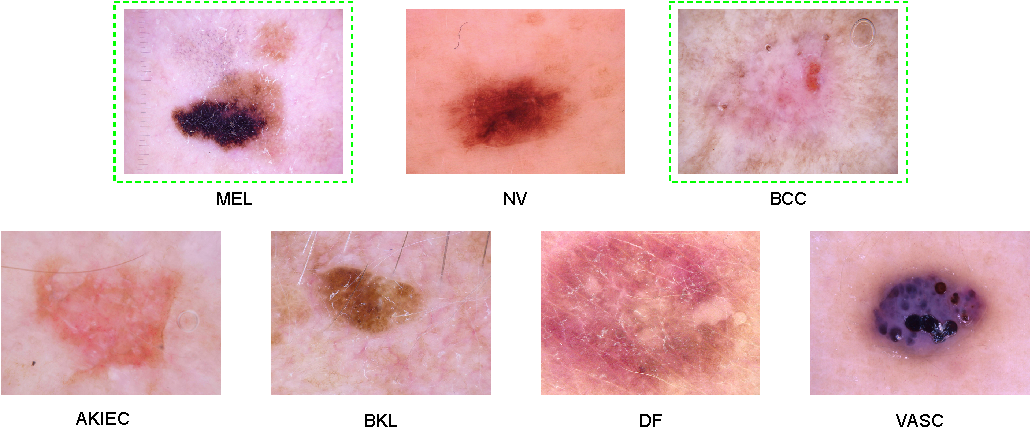
\includegraphics[width=4.2in]{mel}
		\caption{Samples of each type of skin lesion from the ISIC 2018 dataset, where BCC and MEL are skin cancers (in the green dotted box), and others are common skin diseases\cite{codella2019skin}.}
		\label{Fig:mel} 
\end{figure}

In our work, I selected only 200 images from ISIC-2017\cite{codella2018skin}, half benign and half malignant, to ensure balanced categories in Paper I. In Paper II, the dataset was obtained from the University of Salerno, which collaborates with the University of Naples; this dataset has been accurately labeled by experts. Though there were only around 1,000 images, all of them have very high-quality annotations. I developed a CNN model-based 7-point skin lesion malignancy checklist, training, and testing it with the publicly available dataset Dermoscopy Atlas \cite{argenziano2000interactive} dataset, which contains 1011 dermoscopic images.


\begin{table}[!htbp]
\centering
\caption{The 7-point checklist criteria with related
individual scores.}\label{tab:point}
\begin{tabular}{p{9cm}c}
\toprule
\rowcolor{dGray}
\textbf{Clinical features}& \textbf{Score}\\
\midrule
\rowcolor{Gray}
\textit{Major criteria} &\\ 
%\rowcolor{gray!40}
\rowcolor{Gray}
Atypical pigment network & 2\\
\rowcolor{Gray}
Blue-whitish veil & 2\\
\rowcolor{Gray}
Atypical vascular pattern & 2\\
\midrule
\rowcolor{Lightgrey}
\textit{Minor criteria} & \\
\rowcolor{Lightgrey}
Irregular streaks & 1\\
\rowcolor{Lightgrey}
Irregular pigmentation& 1\\
\rowcolor{Lightgrey}
Irregular dots/globules & 1\\
\rowcolor{Lightgrey}
Regression structures& 1\\
\bottomrule
\end{tabular}
\begin{tablenotes}
        \footnotesize
        \item \textit{Note: A score of 3 or more is regarded as suspicious.}
      \end{tablenotes}
%\noindent{\footnotesize{A score of 3 or more is regarded as suspicious.}}
\end{table}


\begin{figure}[!h]
\centering
	\includegraphics[width=4.2in]{7point}
		\caption{A diagnostic example of a 7-point checklist,  different structures are present and a score of seven is reached \cite{di2004elm}.}
		\label{Fig:7point} 
\end{figure}

The 7-point checklist is a diagnostic method that requires the identification of  seven dermoscopic criteria, i.e., features were selected for their frequent association with melanoma). These seven features refer both to the chromatic characteristics and to the shape and/or texture of the lesion. Dermoscopic images of a melanocytic skin lesion are analyzed for  evidence of the presence of these standard criteria; from this analysis, a score is calculated; finally, if a total score of three or more is attained, the lesion is classified as melanoma (otherwise it is classified as a benign). As for the individual criteria (see Table \ref{tab:point} and Figure \ref{Fig:7point}), there are three “major” criteria with individual scores of two and four “minor” criteria with individual scores of one.





\section{Image preprocessing}
"Garbage in, garbage out.” This slogan is common in computer science, mathematics in computer science, and machine learning. It refers to a very important point: even the best computer vision models will perform badly if the input data are of low quality. It is always crucial to strive to gather high-quality data for the current task. Additionally, even with high-quality data, preprocessing enables the best outcomes to be attained.

Image acquisition is the initial step in image classification. There are many potential sources of dataset bias in skin lesion imaging. Imaging devices or procedures may lead to specific measurement biases. A bias particularly harmful to clinically relevant automated diagnosis is when the data capture medical interventions. For instance, spurious correlations can appear in skin lesion images due to labeling errors.

Before being used for model training and inference, images usually first undergo image pre-processing. This includes, but is not limited to, resizing, orienting, and color corrections. The purpose of preprocessing is to increase the image's quality so that I can analyze it more effectively. Preprocessing allows us to eliminate unwanted distortions and improve specific qualities that are essential for the application I am working on. An image must be preprocessed for software to function correctly and produce the desired results.

There are several reasons for image preprocessing. First, CNNs' fully connected layers require that all the images be in arrays of the same size. Additionally, model preprocessing may shorten model training time and speed up model inference. If the input images are very large, shrinking their size  will greatly decrease the amount of time needed to train the model without significantly affecting model performance. 

\section{Data augmentation}
During the experiment, overfitting and underfitting are assessed in terms of the training error and test error. During the continuous iterative training process of the deep neural network model, the training error constantly decreases; however, after the test error drops to a certain point, it starts to rise. In Figure \ref{Fig:fit}, $t$ represents an inflection point. Before this inflection point has been reached, the neural network model has not reached the optimal state and the model can be considered underfitted. After the $t$ inflection point has been reached, although the training error continues to decrease, the test error starts increasing. This is because, although the training set fits very well, the model's generalization ability is poor and the test set does not perform well. Therefore, the model can be regarded as overfitted. In the case of poor model fitting, adding artificial data through data augmentation can effectively improve the effect of the network model.

\begin{figure}[!h]
\centering
	\includegraphics[width=3.2in]{overfit}
		\caption{Error during training and testing.}
		\label{Fig:fit} 
\end{figure}


Data augmentation is a manipulation applied to images to create different versions of similar content in order to expose the model to a wider range of training examples. For example, randomly altering the rotation, brightness, or scale of an input image requires that a model consider what an image subject looks like in a variety of situations.

Data augmentation manipulations are forms of image preprocessing, but there is a critical difference: while image preprocessing steps are applied to both training and test sets, image augmentation is only applied to the training dataset. Thus, a transformation that could be an augmentation manipulation in some situations may best be a preprocessing step in others.

\begin{figure}[!h]
\centering
	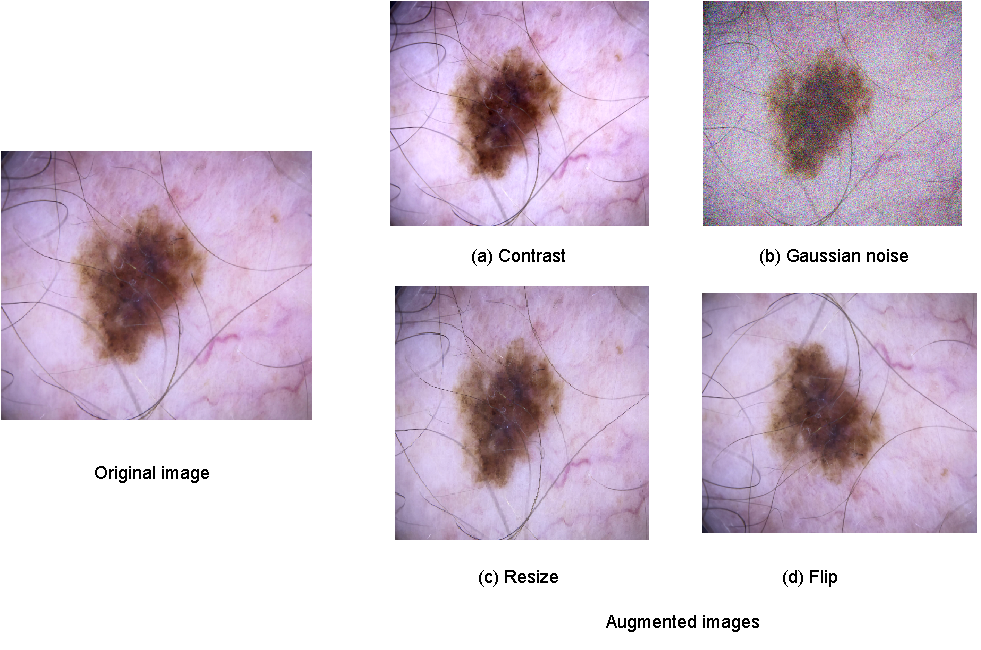
\includegraphics[width=4.2in]{aug}
		\caption{The difference between the original skin lesion image (left) and the images after data augmentation (right).}
		\label{Fig:aug} 
\end{figure}

It is impossible to truly capture an image that accounts for every real world scenario a model may encompass. This is where augmentation can help. By augmenting the images, I can increase the sample size of the training data and add new cases that might be hard to find in the real world. Augmenting existing training data to generalize to other situations allows the model to learn from a wider range of situations. This is particularly important when collected datasets may be small. A deep learning model will (over)fit to the examples shown in training, so creating variation in the input images enables the generation of new, useful training examples.


\section{Convolutional neural networks}  \label{sec:volumetric}
CNNs have the advantage of non-linear mapping by automatically adjusting the training weights between neurons. The standard CNN is basically composed of three layers: the convolutional, pooling, and fully connected layers. Figure \ref{Fig:vgg16} depicts the detailed structure of a Vgg-16 backbone network. The convolutional layer is the most important layer and performs most of the computation. It consists of kernels, which are composed of weights that learn visual features from the input images. Each kernel is convolved across the whole image and produces a feature map, which is the output of this layer. The pooling layer is basically used to reduce the feature map size. Consequently, it reduces the number of training parameters for the next layers, helps control overfitting, and, along with a non-linear activation filter, incorporates non-linearity into the network. The fully connected layer is a standard neural network that is connected to the last feature map provided by the previous layer. In summary, the composition of the convolutional and pooling layers is known as the feature extractor, and the fully-connected layer is the classifier.

\begin{figure}[!h]
\centering
	\includegraphics[width=4.2in]{VGG16_new}
		\caption{Illustration of the backbone network (Vgg-16) used to classify skin cancer images. First, the image features are extracted by the CNN feature extractor. Next, these features are reduced by the pooling layer. Finally, the softmax layer serves as the output layer of the model to predict skin lesion classes. \cite{haris_iqbal_2018_2526396,simonyan2014very}}.
		\label{Fig:vgg16} 
\end{figure}
%map of contributions to goals of research studies

CNNs have emerged as a powerful classification tool and are consistently used in object classification competitions, including the ImageNet challenge \cite{russakovsky2015imagenet}. Since AlexNet \cite{krizhevsky2017imagenet}, using CNN architecture, won the annual ILSVRC in 2012, CNN models such as Vgg\cite{simonyan2014very}, GoogLeNet\cite{szegedy2015going}, and ResNet\cite{he2016deep} have performed well in image recognition and classification. 

Different CNN architectures have been used to deal with skin cancer detection, and successful results have been reported by Steve et al. \cite{esteva2017dermatologist}. Nonetheless, for medical tasks, collecting a large number of data to train a CNN is challenging. To overcome this issue, most research has used transfer learning, a well-known technique in which a model trained for a given source task is partially reused for a new target task \cite{menegola2017knowledge}. In this way, models can be initialized using the weights from the ImageNet dataset \cite{russakovsky2015imagenet} and then fine-tuned using their own dataset. In our work, Paper \uppercase\expandafter{\romannumeral1} used Yolo1, Yolo2, and Yolo3; Paper \uppercase\expandafter{\romannumeral2} used Vgg-16; Paper \uppercase\expandafter{\romannumeral3} used GoogleNet, Inception-v3, and ResNet-101; Paper \uppercase\expandafter{\romannumeral4} used Vgg-19, ResNet-101 and Inception-V3; and Paper \uppercase\expandafter{\romannumeral6} used Resnet-50 as the baseline. These deep learning backbones are based on CNNs and are widely used in computer vision.

\section{Transformer neural networks}  \label{sec:trans}

A transformer model is a neural network that learns context and thus meaning by tracking relationships in sequential data such as the words in this sentence. The transformer neural network was first proposed by Vaswani et al. \cite{vaswani2017attention} in 2017 to solve some sequence-to-sequence tasks while handling long-range dependencies with a simple recurrent neural network (RNN). Vaswani et al. introduced an encoder-decoder architecture based on attention layers, which was called the transformer. Transformer models apply an evolving set of mathematical techniques, called attention or self-attention techniques, to detect subtle ways even distant data elements in a series influence and depend on one another.

Vision transformers (ViTs) use positional encoders to tag data elements coming in and out of the network. Attention units follow these tags, calculating a kind of algebraic map of how each element relates to the others. Attention queries are typically executed in parallel by calculating a matrix of equations in what is called multi-headed attention, as shown in detail in Figure \ref{Fig:trans}.

\begin{figure}[!h]
\centering
	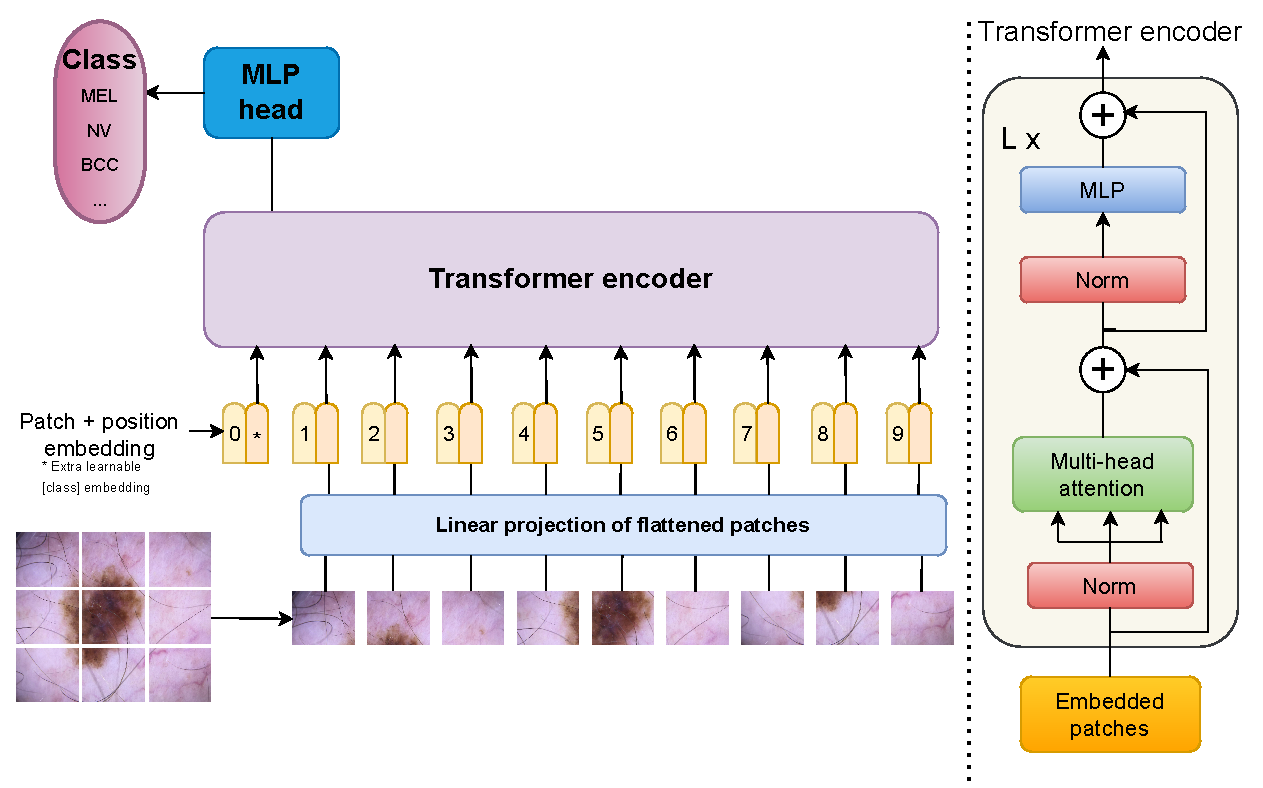
\includegraphics[width=4.2in]{transformer}
		\caption{ViT model overview. The model splits an image into fixed-size patches, linearly embeds each of them, adds position embeddings, and feeds the resulting sequence of vectors into a standard transformer encoder. To perform classification, it uses the standard approach of adding an extra learnable “classification token * ” to the sequence \cite{dosovitskiy2020image}.}
		\label{Fig:trans} 
\end{figure}


Transformers are in many cases replacing convolutional and recurrent neural networks (CNNs and RNNs), the most popular types of deep learning models just five years ago \cite{whattran}. Before transformers arrived, users had to train neural networks with large labeled datasets that were costly and time-consuming to produce. By finding patterns between elements mathematically, transformers eliminate that need, making available the trillions of images and petabytes of text data on the web and in corporate databases. In addition, the math that transformers use lends itself to parallel processing, so these models can run quickly.

 A multi-head self-attention layer with a sufficient number of heads is at least as expressive as any convolutional layer \cite{cordonnier2019relationship}. However, pure transformer networks lack the inductive bias of CNNs and thus need to rely on large-scale data to achieve results comparable to those of CNNs. In Paper \uppercase\expandafter{\romannumeral6}, I used the hybrid Resnet-50 + Transformer model, which achieved good experimental results. In this paper, the input images were first passed through Resnet-50, and then the feature maps were sent to the transformer block. In this process, CNN can capture local features while Transformer will capture global features.

 






\chapter{Summary of publications} \label{ch:method}
This research on skin cancer classification based on deep learning is supported by six papers, the full-text versions of which are available in Part B. This chapter presents a short summary of how these papers support the thesis, as well as the author's contribution to each paper.

\begin{figure}[!h]
\centering
	\includegraphics[width=4.2in]{map}
		\caption{Research objectives, studies, and contributions of the work.}
		\label{Fig:paper} 
\end{figure}
%map of contributions to goals of research studies

\section*{Paper I}
\textbf{Automatic Detection of Melanoma with Yolo Deep Convolutional Neural Networks}, \textit{in 2019 E-Health and Bioengineering Conference (EHB)}



~\\

Paper I addresses the small dataset problem while striving to maintain diagnostic accuracy. In Paper I, only 200 pictures were used to train the model. Yolo is a popular framework for object detection and is effective for the diagnosis of skin diseases. It not only can classify skin diseases, but also can determine the specific location of the lesion. There are three most important features of the Yolo algorithm: first, using a grid instead of a single window moving across the image; second, reducing the complex problem of classification and localization of an object to one regression problem; third, very effective generalization of knowledge. Yolo treats the detection and classification problems as a single regression problem, which puts a grid with the size of $S \times S$ on the image. For each cell of the grid, Yolo predicts whether there are objects in it and for each of them the coordinates of the rectangle surrounding the object are determined. So far, Yolo has been upgraded to eight versions, but I only used three versions at that time. The contribution of Paper I to the whole thesis is to address a small database pain point in deep learning. 

\section*{Paper II}
\textbf{Deep Melanoma classification with K-Fold Cross-Validation for Process optimization}, \textit{in 2020 IEEE International Symposium on Medical Measurements and Applications (MeMeA)}



~\\

Paper II proposes the application of a convolutional neural network-based method using K-fold cross-validation to a small skin disease database. K-fold is a validation technique in which it splits the data into $k$-subsets and the holdout method is repeated $k$-times where each of the $k$ subsets is used as a test set and other $k-1$ subsets are used for training purposes. Then the average error from all these $k$ trials is computed, which is more reliable as compared to the standard handout method. This dataset comes from the University of Salerno, which collaborated with local hospitals to collect data. The data quality is therefore high, although the data volume is relatively small. This dataset contains around 1,000 images and all annotations were made by experts. To improve the diagnostic accuracy, I used a five-fold cross-validation training dataset with Vgg-16 as the backbone to train the data. Cross-validation helps to reduce bias and therefore stabilize performance between the training dataset and the testing dataset.
 

\section*{Paper III}
\textbf{Ensembling CNNs for dermoscopic analysis of
suspicious skin lesions}, \textit{in 2021 IEEE International Symposium on Medical Measurements and Applications (MeMeA)}



~\\

Paper III focuses on improving diagnostic accuracy and using ensembling CNNs as feature extractors to diagnose suspicious skin lesions. GoogleNet, Inception-v3, and ResNet-101 were used here. The dataset used is a public dataset created according to the 7-point checklist standard and containing 1,011 images. Dermatologists usually use the weighted 7-point checklist based on pattern analysis as a diagnostic guide. Here, let the machine combine deep learning and the perspective of a dermatologist to study the skin lesion dataset. In this paper, binary classification was performed on this dataset. The classifier used the "or rule" and the majority decision. In the Datasets section of Chapter \ref{ch:theory}, I have introduced the 7-point checklist in detail. 


\section*{Paper IV}
\textbf{Skin Cancer Classification based on Cosine Cyclical Learning Rate with Deep Learning}, \textit{in 2022 IEEE International Instrumentation and Measurement Technology Conference (I2MTC)}



~\\

Paper IV also focuses on improving diagnostic accuracy. It used three different learning rates for training, while using three different backbones, i.e., Vgg-19, ResNet-101, and Inception-V3. The learning rate is one of the most important hyperparameters when it comes to training a neural network. It determines the magnitude of weight updates. It is also the trickiest parameter to set because it can significantly impact model performance. Cyclical learning rates enable learning rates to oscillate back and forth between a lower and upper bound. The benefits are that have more freedom in initial learning rate choices and break out of saddle points and local minima. The dataset used is the large Ham10000 dataset.

\section*{Paper V}
\textbf{Recent Advances in Diagnosis of Skin Lesions Using Dermoscopic Images Based on Deep Learning}, \textit{in 2022 IEEE Access}



~\\

Paper V  is mainly a literature review of the research on deep learning for skin disease diagnosis published between 2017 and 2022. This paper presents the challenges of melanoma classification based on dermoscopic images, reviews common methods and novel methods to improve accuracy, and offers guidance for future research directions. This paper present and summarize the latest methodology in melanoma classification and the techniques to improve this. It discusses advancements in deep learning-based solutions to diagnose skin cancer, along with some challenges and future opportunities to strengthen these automatic systems to support dermatologists and enhance their ability to diagnose skin cancer.

\section*{Paper VI}
\textbf{A Deep CNN Transformer Hybrid Model for Skin Lesion Classification of Dermoscopic Images using Focal Loss}, \textit{in 2022 MDPI Diagnostics}



~\\

Paper VI proposes a CNN Transformer hybrid model in an end-to-end fashion incorporating a focal-loss based loss function to classify skin lesion images. If the selected neural network is too deep, due to the limited number of training set samples used, 
this leads to overfitting of the network, but underfitting occurs if the network is chosen to be too shallow. This conclusion has been verified in many experiments. After multiple data enhancement experiments and comparisons, the LeNet network model has an accuracy of about 76$\%$ in the classification of skin cancer images, the AlexNet model an accuracy of about 79$\%$, the GoogLeNet model an accuracy of about 83$\%$, and the ResNet network model a stable accuracy of 85$\%$. Therefore, this paper chose the ResNet model because of its better image classification. Currently, the mainstream ResNet model is divided according to the depth of the network, there being four types: ResNet-50, ResNet-101, ResNet-152, and ResNet-200. Since the networks of ResNet-152 and ResNet-200 are too deep, the training is time-consuming, and when the network model layers are too deep, a large number of data is required to derive the training parameters. The size of the training set in this paper was limited, so only the ResNet-50 network model was selected for the experiment.

In general, the focal loss function is chosen as it is more appropriate for counting the contributions of samples that are difficult and easy to classify, respectively, to the total loss. The underlying idea of the focal loss function was regarded as especially suitable for the research content of this article. Through the focal loss function, the contribution of easily misclassified malignant melanoma images 
 to the total loss can be increased, and the relatively large number of benign skin diseases that are easily classified can be reduced. %The contribution of the image to the total loss.
% \begin{figure}
% \centering
% 	\includegraphics[width=2.2in]{figures/ddist2.png}
% 		\caption{Flying altitude.}
% 		\label{Fig:side} 
% \end{figure}


% % In this placement, every dome inscribes a regular hexagon, such that its sides are equal to $r$. The overlapping between each two domes has a length of $r$ and height ,$h$, of $\frac{1}{2}\times r$.

% In this placement, every three adjacent noncollinear domes form an equilateral triangle. Its side, $s$, is the distance between the centers of the two adjacent domes, Fig. \ref{fig:before}. That distance equals to $2 \sqrt{(r^2)- (h^2)}$.
% and its altitude, $t$, equals to $\frac{\sqrt{3}}{2} \times s$.
% This placement provides full coverage on the ground level. In 3D volume, intersection points of every three adjacent noncollinear domes would be blind spots with zero coverage at the flying altitude as shown in Fig. \ref{fig:before}. Therefore, domes should be re-positioned in order to provide full coverage at the defined altitude. 


% In order to cover the blind spots while keeping the thinnest hexagonal pattern, the altitude $t$ should be reduced by $d$ in Fig. \ref{Fig:side}. Therefore, the new triangle side $s'$, which represents the distance between domes center, is equal to: 

% \begin{equation} \label{eq:dist}
%   s' = s - 2d /\sqrt{3}
% \end{equation}
% Re-positioning the domes provides full coverage of the volume, including intersection points as shown in Fig. \ref{fig:after}. It also changes the minimum overlapping height, $h$, between adjacent domes that ensure 100\% detection at flying altitude $a$. This height can be calculated as the apothem of the equilateral triangle, which equals to:

% \begin{equation} \label{eq:height}
%     h = t/3
% \end{equation}

% \begin{figure*}[h]
  
%     \subfloat[Thinnest covering with blind spots ]{{\includegraphics[width=0.49\linewidth,height=2in]{figures/place-before2.png}
%     \label{fig:before}}}
%     %\hspace{0.5em}
%     \subfloat[Full coverage placement]{{\includegraphics[width=0.49\linewidth,height=2in] {figures/place-after3.png}
%     \label{fig:after}}}
 
%     \caption{Hexagonal placement of camera domes.}
%     \label{fig:place2}
% \end{figure*}
% The flying altitude is used as a constraints to re-position while guaranteeing 100\% detection. In Fig. \ref{Fig:place2}, 


% Two placement constraints defined are, the dome capacity and the maximum flying altitude $a$. The dome capacity is obtained from its coverage radius $r$ multiplied by the minimum pixel resolution required for detection at that distance. For example, if the coverage radius of the dome is 500 meters and the required minimum detection resolution is 10 pixels at 500 meters, then the dome capacity is 5000.
% %pixels per meter (pix/m).
% The flying altitude $a$, should not be more that $r$, in order to ensure that the object is detected all the time it is flying within the covered volume. 
% We used the flying altitude as a constraints to calculate how much to move the nodes to cover the blind spots



% \begin{figure}
% \centering
% 	\includegraphics[width=0.5\linewidth,height=3in] {figures/placement.pdf}
% 		\caption{Coverage blind spot in hexagonal placement}
% 		\label{Fig:blind} 
% \end{figure}

% \begin{figure}
% \centering
% 	\includegraphics[width=\linewidth]{figures/placement1.png}
% 		\caption{Blind coverage spot when the direct application of hexagonal placement}
% 		\label{Fig:place1} 
% \end{figure}


% \subsection{Placement Evaluation}

% The optimized placement method discussed in \ref{sec:hexa} should achieve 100\% detection for any object flying withing the defined flying altitude. Overlapping coverage between camera domes allows extracting object
% stereoscopic information such as size and position. These criteria should be measured in order to assess the multi-camera placement.

% The method developed in \cite{paper1} evaluates coverage effectiveness of each dome placement in volumetric surveillance. Three monitoring objectives are defined and measured using GPS trajectories of six birds over an area of 9 $km^2$. The tracks are obtained from the work in \cite{birdstracks}. The defined criteria are detection, and positioning
% percentage of flying object; as well as the maximum pixel
% resolution captured to detect it.

% The required minimum detection resolution and the dome coverage radius define the dome capacity, Eq. \ref{eq:capacity}. Each tack composes of number of samples representing the coordinates in longitude and latitude. The altitude is assumed to be 200 meters for all tracks. These coordinates are converted to a Euclidean distance vector corresponding to each track. The dome capacity is then used to calculate the pixel resolution of each sample in the distance vector. 

% \textit{Detection percentage}, is calculated for each tack when its pixel
% resolution is higher than the required detection resolution. The defined resolution is 3 pixels per meters ($pix/m$). Whenever this resolution is fulfilled for the object flying over any of the domes, it means the object is detected. The placement method in \ref{sec:hexa} ensures 100\% detection for the six used trajectories over the defined 9 $km^2$ volume. Also, when the object detected in two domes, its position can be extracted. The \textit{positioning percentage} measures that when the birds fly withing overlapping areas. Moreover, the pixel resolution to detect the object changes as it flies closer or further the dome center. The \textit{maximum pixel resolution} gives an indication of that. 


% \section{Node Configuration}
% The aspect of optimizing surveillance system includes at its core the node optimization. To achieve that, two factors are considered; cost of the multi camera dome, \cite{paper3}, and its design, \cite{paper4}. 

% \subsection{Node Design Exploration}

%  The multi-camera dome is assumed to consist of multiple layers vertically and each layer consists of number of cameras at the horizontal level as in Fig. \ref{Fig:dome3d}. The design exploration in \cite{paper3} construct a cost efficient camera dome, subject to monitoring constraints, from a set of camera sensors and lenses combination. The combined horizontal angles of the cameras
% in one layer should cover a minimum of 360$^\circ$. The vertical
% angles of all the layers combined should cover a minimum of
% 90$^\circ$ to ensure monitoring a 2$\pi$ radian view. Cameras in one layer are identical, however it is not necessary that all layers have similar cameras. 

% %Therefore, we can assume that the dome is more than one layer, as shown in Fig. \ref{Fig:dome3d}. 

% \begin{figure}
% \centering
% 	\includegraphics[width=0.7\textwidth, height=2.1in]{figures/dome3d.pdf}
% 		\caption{Multi-camera dome architecture.}
% 		\label{Fig:dome3d} 
% \end{figure}

% For the design exploration, a number of constraints are defined. They include, the dome coverage radius, $r$, the minimum pixel resolution at distance $r$, and number of layers in the node. The method searches through available
% sensors and lenses to combine them such that the diameter of the covering lens must be equal or larger than the sensor size. Then, an exhaustive search algorithm is performed using the short-listed combinations. Each sensor-lens pair should fulfill pixel resolution constraint at the specified dome radius. The solution with the minimum cost is chosen as optimal. The search for optimal solution can be constrained for example by cost, number of cameras, or other parameters. The optimal solution has the following properties, the angle covered by all the layers vertically, total number of cameras in the node, number of cameras in each layer, and the solution cost. 

% % This method also investigates trade-offs among design parameters and constraints
% % to achieve the optimal solutions.
% The method estimates the cost of each member, $S_{ijn}$, of the solution space, $S$, subject to the defined design constraints. The objective function for the design exploration can be defined as minimizing the following cost function: 

% \begin{equation}\label{eq:costf}  
% \begin{aligned}
% & \underset{ \tilde{C}_{ijn}}{\text{minimize}}
% & & f( S ) \\ %\mathrm{f}
% & \text{subject to}
% & & d^c_i \leq d^o_j, \\ 
% &&& M_{ijn} \leq M, \\
% &&&  N \leq L, \\
% & & & \delta_{rijn}  \geq \delta, \\
% & & & A_{ijn} \geq \frac{\pi}{2} + \varepsilon \cdot (N-1) 
% \end{aligned}
% \end{equation}
% where $d^c_i$ and $d^o_j$ is the diameter of sensor and the covering lens, respectively, $M_{ijn}$ is the number of cameras required by the solution, 
% $A_{ij}$ is the total vertical angle covered by all layers, $N$, and $\delta_{rijn}$ is the pixel resolution in the optical plane of the FoV for the combination of camera $i$ and lens $j$ at distance $r$ from the dome for each layer $n$ in the solution.

% \subsection{Node Cost Optimization} \label{sec:cost}
% The optimized placement method in \ref{sec:hexa} motivates the inclusion of the placement in the node design. In the hexagonal placement, domes overlap in order to achieve full coverage. Also, volumes above the monitoring height are not required to be monitored. This results in coverage overhead as shown in Fig. \ref{Fig:overa}. Moreover, the coverage of each dome without the overlap in the hexagonal pattern can be modeled as a hexagon, Fig. \ref{Fig:overb}.

% \begin{figure*}
% \centering
% \subfloat[Side view]{\includegraphics[width=2.7in, height=1.3in]{figures/fig3b.png}%
% \label{Fig:overa}}
% \hfil
% \subfloat[Top view]{\includegraphics[width=1.5in]{figures/fig3a.png}%
% \label{Fig:overb}}
% \caption{Coverage of multi-camera domes in hexagonal placement.}
% \label{Fig:overhead}
% \end{figure*}
% % \begin{figure}
% % \centering
% % \includegraphics[width=3in, height=1.3in]{figures/fig3b.png}%
% % \caption{Coverage overhead in hexagonal placement.}
% % \label{Fig:overhead}
% % \end{figure}

% Taking these points into account leads to changes in node design in order to avoid coverage overhead in the hexagonal placement. Therefore, in \cite{paper4} the hemispherical design of the node is optimized accordingly. The monitored volume for each dome is
% modeled as a cylinder instead of a hemisphere, Fig. \ref{Fig:cylinder:b}. Non-overlapping volumes have a minimum
% coverage radius equals to the monitoring height. Overlapping volumes coverage radius is be bounded by the cylinder radius, $r_c$. The resulting cylindrical dome is then divided into layers, and each of them has its coverage radius. Monitoring requirements should be met at that distance. At the top layer, cameras are stacked with multiple overlap at the horizontal level. This also causes coverage overhead. Therefore, only one camera can be mounted at the top layer, Fig. \ref{Fig:cylinder:a}. That layer can be considered as a half layer when arranging the layers vertically from bottom up to cover a minimum of 90$^\circ$.
% The minimum coverage radius of each layer is defined based on the monitoring height, $h$. 

% \begin{equation}
%   {{r}_{L}}=\begin{cases}
%     {{r}_{c}}/\cos (c_A), & \text{if $x\And y<h$}.\\
%     {{r}_{m}}, & \text{if $x>h\And y<h$}. \\
%     h/\sin (p_A), & \text{if $x\And y>h$}.
%   \end{cases}
%     \label{eq:9}
% \end{equation}
% where x and y are height of the current and previous layer respectively, as shown in Fig. \ref{Fig:cylinder:b} for layer 2. ${c_A}$ is the covered vertical angle of the current and previous layers. ${p_A}$ is the vertical angle of view of the previous layer. The vertical angle of view for each layer is calculated as:

% \begin{equation}
%  v_A=2\arctan ({{d}_{v}}/2f)
%   \label{eq:11}
% \end{equation}
% where ${{d}_{v}}$ is the sensor's vertical dimension and $f$ is the lens focal length. Each layer's height is calculated as:
% \begin{equation}
%   {h}_{L}=|{{r}_{m}}.\sin ({c_A)}| 
%       \label{eq:10}
% \end{equation}

% \begin{figure*}
% \centering
% \subfloat[]{\includegraphics[width=1.0in]{figures/fig5a.png}%
% \label{Fig:cylinder:a}}
% \hfil
% \subfloat[]{\includegraphics[width=2.8in]{figures/fig5b.png}%
% \label{Fig:cylinder:b}}
% \caption[Optimized cylindrical dome design]{(a) Camera's field of view in 3D, (b) Optimized cylindrical dome design with one camera on the top layer. }
% \label{Fig:cylinder}
% \end{figure*}

% \section{Object Detection and Positioning}
% For the problem of sky monitoring in wind farms, object detection is an essential surveillance task. To investigate methods for in-flight birds detection, the performance of state of the are deep learning YOLOv4, \cite{yolov4}, is compared to computer vision based detection using background subtraction. An improved YOLO-based model is developed in \cite{paper6} and it achieves detection accuracy on testing sets of 90\% and 92\% using the datasets in \hl{dataset}\cite{mydataset}.

% %\subsection{Background subtraction}
% \subsection{Deep Learning based Object Detection}
% \subsubsection{Dataset Acquisition:}
% Object detection using deep learning requires annotated datasets for
% training, validation, and~testing. There were not any available datasets for in-flight bird that can be used in this study. Therefore, datasets were collected by Mid Sweden university in two wind farms in Denmark over the
% course of a few months in 2017 and 2018. The datasets were manually annotated using the open source annotation tool \textit{LabelImg}, \cite{labelimg}.

% \begin{figure}
%  \includegraphics[width=0.99\linewidth]{figures/dataset.pdf} 
% \caption[Example frames from Skagen and Klim datasets]{Frames from Skagen dataset (left), Klim dataset (middle), and examples of birds from both datasets with the corresponding pixels count for each box (right).}
% \label{Fig:datasets}
% \end{figure}

% \begin{figure}
% \centering
% \subfloat[]{\includegraphics[width=0.45\linewidth,height=1.5in]{figures/skagen-hist.png}%
% \label{Fig:skagen}}
% \hspace{0.3cm}
% \subfloat[]{\includegraphics[width=0.45\linewidth,height=1.5in]{figures/Klim-hist.png}%
% \label{Fig:klim}}
% \caption[Bird size statistics from Skagen]{Bird size statistics from Skagen (a) and Klim (b) datasets.}
% \label{Fig:histos}
% \end{figure}

% The Skagen dataset was collected at the \textit{Skagen Grey Lighthouse, Center of Migratory Birds} using a pair of wide-angle monochrome
% cameras fixed inside rigid boxes. The cameras were connected to
% Nvidia Jetson TX2 edge-computing device recording $4K$ images at
% $5\ fps$. This dataset has relatively stationary background, in terms of clouds movement and illumination, Fig. \ref{Fig:datasets} (left). Majority of objects size in Skagen dataset are less than $200$ pixels, Fig. \ref{Fig:skagen}, which are considered very small. This dataset was used mainly to test the deep learning model, rather than training it.

% The second annotated dataset is Kilm, and it was collected at \textit{Klim Fjordeholme} using the same camera setup; except here the cameras
% were mounted on tripods. This dataset exhibits a more dynamic
% background of moving clouds and variant illumination, Fig. \ref{Fig:datasets} (middle). Objects sizes vary in this dataset as shown in Fig. \ref{Fig:klim}, which makes it good option for training and validation.  



% \subsubsection{YOLOv4-based Models:}
% At the time this study was conducted, the state of the art in deep learning based object detection is YOLOv4. When the network was trained using full resolution frames ($3840 \times 2160$) form Klim dataset, the model missed most of the small objects, False Negatives (FN). This happens because frames get resized into the specified width and height of the network architecture during training, $1024 \times 1024$. When objects are already small and the frame get resized, pixel information get lost and as a results the model does not learn from these examples and consequently does not detect them during inference. In Fig. \ref{fig:models}, this model is referred to as Model 1.

% \begin{figure} [t]
% \includegraphics[width=\linewidth,height=3.3in]{figures/models-combined2.pdf}
% \caption[Three YOLOv4 based models]{Three YOLOv4 based models, each trained on the Klim dataset, for birds detection around wind farms.}
%   \label{fig:models}
% \end{figure}

% To address the problem of small objects in 4k resolution, Model 2 splits the input frames into four frames of $1020 \times 1080$ before feeding them to the network, Fig. \ref{fig:models}. The frames are then resized to the network width and height. This model detects small birds better compared to Model 1, since number of FN (missed detections) decreases. It is assumed that birds at the tiling
% boundaries are a rare occurrence, also that birds do not stay long at these areas of the frame. Therefore, birds striding one of the four tiling boundaries is left as future work.

% Frames in the dataset used for training are extracted from a video sequence. Which means that temporal information from successive frames are connected. Incorporating temporal in addition to the
% spatial information of objects across multiple frames, allows
% the network to learn objects more accurately and differentiate them from
% noise since objects will appear in successive frames. Frames in both datasets are 24-bit grayscale, such that each pixel has three channels R, G, and B. For each frame at time $t$, Model 3 uses R and B channels to store pixel values of the object in the previous and next frame at time $t-1$ and $t+1$, respectively, before feeding it to the model for training. Model 3 also uses tiling similar to Model 2. Therefore, given 3 4K images, four $1920 \times 1080 \times 3$ tiles are constructed. Each
% of them is then resized to $1024 \times 1024 \times 3$ and passed into YOLOv4 network. Utilizing temporal features in Model 3 is shown in \ref{fig:models}.

% \subsubsection{Training Parameters:}

% To train the three models using the custom Klim dataset, transfer learning was used. Training starts using YOLOv4
% weights pre-trained on the MS COCO dataset. The used weights file is yolov4.conv.137, which freezes the wights up to convolutional layer number 137, one layer before the first YOLO layer, and train the rest of the layers using the custom dataset. The models were trained using Google Colab Pro cloud services, alternating between
% Tesla P100-PCIE and V100-SXM2 16GB GPUs

% The network configuration includes number of hyper parameters. A grid search is performed to find optimal values for the following parameters: batch size, subdivision, network resolution, learning rates, and anchors. These parameters are set set as: batch size: 64, sub-division: 32, height and width: 1024, momentum: 0.949, learning rate: 0.001, decay:
% 0.0005, and max batch: 2000. As the dataset has only one class, the number of
% filters before each of the three YOLO layers is set to 18. The hyper parameters for each model are defined in Table \ref{tbl:training-parameters}.

% \begin{table} [h]
%  \caption{Training parameters for Model 1, 2 and 3.}
%  \label{tbl:training-parameters}
%  \small
%  \resizebox{\textwidth}{!}{% 
% \begin{tabular}{p{1.2cm}p{2.7cm}p{3cm}p{3cm}} 
%   \toprule 
%     & \textbf{Model 1} & \textbf{Model 2} & \textbf{Model 3} \\ \toprule
    
%      burn in &  100 & 400 & 400 \\ \midrule
%      steps & (1600, 1800) & (1400, 1700) & (1400, 1700) \\ \midrule
%      scales & ({0}.1, {0}.1) & ({0}.1, {0}.01) & ({0}.1, {0}.01) \\ \midrule
     
%      anchors & (4,5) (6,7) (9,9) (8,14) (14,12) (15,20) (24,25) (32,46) (74,121) 
%      & (5,8) (7,11) (11,13) (13,18) (20,18) (20,29) (33,27) (50,47) (60,98)
%      & (5,8) (7,11) (11,14) (15,17) (21,20) (19,31) (32,27) (48,46) (61,97)\\
% \bottomrule
% \end{tabular}}
% \end{table}

% \subsection{Object Positioning}

% The calibrated stereo vision system in \cite{paper5} is used to obtain precise positions of objects using two projection levels. The system is constructed of two stereo pairs, each has two cameras, Fig. \ref{Fig:Deployment2}. The cameras were calibrated using artificial LED light as 3D reference points. After calibration, the 2D image coordinates of reference points are calculated using the projection matrix in \ref{eq:projectm}. These points are then back-projected to rays in order to measure the error between the real and projected position. 

% The first level of positioning estimates the object position using its visibility in the first camera pair. The two back-projected rays from camera pair usually do not intersect at the exact position of the object. This is because of cameras alignment and baseline and having the points not at the exact same epipolar line. Therefore, to approximate the closest point to the object, the method in. \cite{midpoint} of finding the mid point is used. 

% The second stage uses the position obtained from the first level and the back projected ray of the point in the third camera. The mid point between these two is calculated as the refined position of the object. This position is closer to the object than the one obtained from the first layer, because the projection error is smaller. The re-projection error is calculated as:

% \begin{equation}\label{eq:error3d}
% 	\epsilon_r  = \sum_{i=1}^{n}\frac{\sqrt{(\hat{X_{i}} - X_i)^2+(\hat{Y_{i}} - Y_i)^2+(\hat{Z_{i}} - Z_i)^2}}{n}
% \end{equation}
% where $(X_{i}, Y_{i},Z_{i})^T$ are the ground truth point coordinates in 3D and  $(\hat{X}_{i}, \hat{Y}_{i},\hat{Z}_{i})^T$ are reconstructed coordinates of the same points.

% \begin{figure}
% \centering
% 	\includegraphics[width=2.9in, height=3in]{figures/deployment.png}
% 	\caption{Deployment of two layers positioning.}
% 		\label{Fig:Deployment2}
% \end{figure}
\chapter{Discussion} \label{ch:results}

In this chapter, I mainly discuss the use of small datasets in deep learning and some methods to use when the data are imbalanced with multiple classes. The ensemble and hybrid models are also discussed, and finally, discuss some remaining challenges and future trends are presented.

\section{Small datasets with deep learning}
Deep learning models are notorious for their data appetite. The more data one can give them, the better they perform. Unfortunately, in most real-life situations, this is impossible in most real-life situations. One may not have enough data, or the data may be too expensive to collect. Luckily, there are several techniques that can be used if one runs short of data. There are basically two methods, i.e., transfer learning and data augmentation, that can help train deep learning models with small datasets. These techniques can help build a deep learning model that can generalize well. In Paper \uppercase\expandafter{\romannumeral4}, I applied transfer learning for skin lesion classification, by first training a model on the ImageNet dataset, and then retraining it on the HAM10000 dataset that has fewer data. In both papers \uppercase\expandafter{\romannumeral4} and \uppercase\expandafter{\romannumeral6}, I  used data argumentation to increase the diversity of the data without actually having to collect new data.

Generative Adversarial Networks (GANs) \cite{goodfellow2020generative}, are ML models capable of generating data. They consist of two competing artificial neural networks: one (the generator) has the task of generating real-looking data, while the other ( the discriminator) classifies the data as real or artificial. In a competition between the generator and the discriminator, the generator tries to generate data sets that the discriminator considers to be real. The discriminator's goal is to recognize the artificially generated data and distinguish it from real data. The generator and discriminator constantly try to "outsmart" each other. Through constant learning and many iterations, the generated data becomes better and better. In our work, the GAN method is not used to generate skin lesion images. 

\section{Methods for addressing data imbalance}

Imbalanced classification samples will not only degrade the performance of traditional machine learning methods but also degrade the performance of deep learning methods. The overall accuracy of image classification is often affected by a large number of samples in the majority class, but in many tasks, the accuracy requirements for the minority class are as important as those for the majority class. For example, in the malignant melanoma classification task studied in ISIC 2016 dataset \cite{gutman2016skin}, the proportions of benign can be as high as 81$\%$ in the training dataset. Therefore, it is particularly important in this study to ensure the accuracy of the minority class while improving the overall classification accuracy.

Researchers mainly use two methods. The first method is to convert unbalanced data into balanced data using "external" methods, such as downsampling or oversampling, so that the training data are balanced, and the classification algorithm does not need to be changed. In contrast, another method is to learn the features more fully from the unbalanced data by adjusting the learning algorithm in the cost adjustment technology without changing the data ratio.

\subsection{Sampling}
 The method of sampling the data set by adding or deleting its features set will change the size of the training set, and both oversampling and undersampling can be used to change the proportions of data in the training set. Oversampling refers to the repeated sampling of small categories of data; in contrast, undersampling refers to the partial sampling of multi-sample categories, for example, the random sampling of part of the data. By oversampling or undersampling, the proportions of samples of different categories in the dataset can be balanced to achieve a better effect. Many experiments can prove that these two sampling methods are effective for addressing data imbalance. However, these two methods also have problems. For example, oversampling increases the size of the training set, and the corresponding training time will increase; at the same time, multiple samplings can lead to overfitting problems because only a few samples are repeatedly trained. Undersampling will discard a lot of useful data. In Paper \uppercase\expandafter{\romannumeral4}, in order to change the imbalance between the categories of data, I used the upsampling method, so that each category has about 5000 images.

 \subsection{Loss function}
 The main idea is to increase the weight of misclassified samples and ignore samples that are easy to classify. The consequences of the imbalance of categories are very influential. The number of negative samples is huge, so in the process of training the neural network, negative samples will account for most of the loss function, and such samples happen to be the easiest to classify. Using this process to optimize the model will therefore not yield the desired results. What I want is that the positive samples of the objects that need to be detected should train the network model more than those background samples.  In Paper \uppercase\expandafter{\romannumeral6}, I chose to use the changing loss of the training model to balance the weights between different classes. Cross-entropy loss is a commonly used image classification loss function, and it is used here as the baseline. I also compared weight cross-entropy and focal loss. Through experimental comparison, I found that focal loss had the best effect.

% \begin{itemize} \label{sec.imb}
    % \item \textbf{Sampling:}
    % \item \textbf{Loss function:} 

% \end{itemize}



\section{Ensemble model and hybrid model}


Strategies using an ensemble of several models\cite{guergueb2022skin,rahman2021approach,ding2022two,kausar2021multiclass,shorfuzzaman2022explainable,mahbod2020transfer} are popular to apply in skin lesion classification. Ding et al. \cite{ding2022two} tested their methods on the ISIC 2017 dataset. They proved that using an ensemble model can improve the results by 6$\%$.   Mahbod et al. \cite{mahbod2020transfer} used a multi-scale and multi-network ensemble model and developed a three-level fusion scheme; in the end, however, their achieved only 86.2 $\%$ accuracy. Using the same ISIC 2018 dataset, our hybrid model with focal loss reached 89.5$\%$ accuracy. Here, an end-to-end CNN Transformer hybrid model was proposed to conduct melanoma classification with dermoscopic images.

In Chapter \ref{ch:theory}, I presented the CNN and ViT approaches.  Inspired by the success of the Transformer network in neural machine translation and of the CNN in computer vision, in our work, I constructed a CNN Transformer hybrid melanoma classification model. CNNs are powerful feature extraction frameworks that are able to learn features from dermoscopic images and can achieve high accuracy in skin lesion classification tasks. However, traditional CNN architecture cannot capture rich global contextual information due to the limits of the CNN receptive field. The transformer architecture utilizes multi-head self-attention modules to represent the sequence patterns \cite{li2020cnn}. ViT can effectively capture long-distance feature dependencies but fails to extract local feature details. The proposed CNN-ViT hybrid model can leverage both global and local information.  The experimental results indicate that our hybrid model is clearly better than the ensemble model.

\section{Existential challenges}

One challenge when comparing skin lesion classification methods is that the problem formulations considered in the individual works differ, although sometimes only slightly. This occurs not only for the training classes and data considered, but also for the  statistical quantities presented. In addition, some works use nonpublic archives of skin clinics in addition to publicly accessible data archives \cite{haenssle2018man,esteva2017dermatologist}, making it even more difficult to reproduce the results.

Since 2016, the ISIC Melanoma Project has attempted to ameliorate this problem  by establishing a publicly accessible archive of dermatoscopic skin lesion images as a benchmark for education and research \cite{gutman2016skin}. In addition, the Project announced an annual challenge in which a clearly defined problem must be addressed. It would be desirable for more work would be compared with this benchmark to achieve a better ranking of the studied procedures and of the state of research. However, the ground truth of the test dataset has not been made public since 2018, making it is difficult to apply this standard benchmark without participating in the challenge.

In addition, it is difficult and often impossible to compare the performance of published classification results, since many authors use nonpublic datasets for training and/or testing. Future publications should use publicly available benchmarks and fully disclose the methods used for training in the interested of comparability.

Cassidy et al. \cite{cassidy2022analysis} found a significant number of duplicate images, both within and between the ISIC datasets. Additionally, they also noted duplicates spread across the testing and training datasets, as shown in Table \ref{dup}. However, in our later experimentation, I discovered that the HAM10000 and ISIC2018 training datasets were the same, and that half of the data were repeated. A good dataset is very important for research, so much so that choosing a good dataset is half of the successful model training.

\begin{table}[!htbp]
\centering
\caption{Number of image files deleted from each ISIC training set after applying our duplicate removal strategy. \cite{cassidy2022analysis}.}\label{dup}
\scalebox{1}{
\begin{tabular}{p{2cm}cccc}
\hline
\textbf{Year} &\textbf{Task no.} &\textbf{Trained} & \textbf{Removed} & \textbf{Remaining}\\
\hline
2016& 3& 900 &826 &74\\
\hline
2017& 3& 2000&801 & 1199 \\
\hline
2018& 3& 10,015&10,015&0 \\
\hline
2019& 1& 25,331&2,235 &23,096\\
\hline
2020& -& 33,126&433 &32,693\\
\hline
Total& -& 71,372&14,310 &57,062\\
\hline
\end{tabular}
}
\end{table}

Another important challenge in this research area is the development of large public image archives comprising images as representative of the world population as possible \cite{navarrete2018automated}. Existing image archives mainly contain skin lesions from light-skinned people. The images in the ISIC database, for example, come mainly from the United States, Europe, and Australia. To achieve accurate image classification for dark-skinned people as well, DL must learn to abstract from the skin color. However, this can only occur if DL observes enough pictures of dark-skinned people during the training.

Collecting higher quality and more images remains a great challenge. For instance,  Pacheco et al. \cite{pacheco2020impact} collected their Dermatological Assistant Program (PAD) dataset for one and a half years, accumulating only 1,612 images.

Due to the large number of parameters in the deep neural networks, if the number of training sets is relatively small, the neural network model will be prone to overfitting, and the generalization ability of new test data is will be poor. It is therefore necessary to better train the network to avoid overfitting. This requires a large number of images in the training datasets; for example, the ImageNet dataset has more than 14 million images as data.

Although an increased number of images for training images will most likely improve the classification accuracy of deep learning algorithms, the number of clinical images that can be collected for certain diseases may be insufficient for this purpose. The ImageNet project is the largest visual database designed for use in visual object recognition software research. The abundant images in ImageNet have become the foundation for the future development of deep learning technology. To further improve the accuracy of such systems, it will be important to increase the number of available clinical images of patients of different ages and ethnicities.

\section{Future trends}

Future work should take these aspects into account. There is a trend toward developing CAD systems embedded in smartphones, either for general users or to assist doctors \cite{chao2017smartphone,ngoo2018fighting}. Using smartphones to assist in skin cancer detection is promising; however, this method requires clinical images instead of dermoscopic ones\cite{pacheco2020impact}. Most of the proposed approaches do not consider patient clinical information, which is important for more accurate diagnosis. In fact, dermatologists do not rely solely on image screening; but also use clinical data to improve their detection accuracy.

\begin{figure}
\centerline{
 \includegraphics[width=\linewidth]{history} 
 }
\caption{The story of AI \cite{bommasani2021opportunities}.}
\label{Fig:his}
\end{figure}

 Improved classification quality could be achieved by adding metadata (e.g., age, gender, race, skin type, and anatomical location) as inputs for the classifiers. This additional information would be advantageous for dermatologists' decision-making, as Haenssle et al \cite{haenssle2018man} have shown.

The application also allows the tracking of all patient lesions to follow their evolution
over time. Evolution is an important consideration, and it is represented by the E in the ABCD(E) rule. Despite its importance, evolution information will take some years to become available, since a lesion may take some time to increase in size and the patient needs to return to the clinic for ongoing assessment. In this context, when the dermatologist asks the patient whether a lesion has increased  in size or changed in form/appearance, s/he is trying to get information about the lesion’s evolution. It is important to note that clinicians collect this information by questioning patients, which may lead to imprecision and uncertainty. Therefore, clinical data must be used to support the diagnosis. The main information is still coming from the image, however.

Regarding the region of the body where the skin lesion is located, Pacheco et al.\cite{pacheco2020impact} grouped all regions into 15 macro-regions that are more frequently encountered and have more potential to raise skin lesions, as follows: face, scalp, nose, lips, ears, neck, chest, abdomen, back, arm, forearm, hand, thigh, shin, and foot. As skin lesions appear more frequently in certain regions of the body \cite{wolff2009fitzpatrick}, this is an important feature to consider.


% \begin{figure*}
% \centering
% \subfloat[]{\includegraphics[width=2.2in,height=2.9in]{figures/paper1-a.png}%
% \label{Fig:paper1:a}}
% \hspace{0.1em}
% \subfloat[]{\includegraphics[width=2.1in,height=2.9in]{figures/paper1-b.png}%
% \label{Fig:paper1:b}}
% \caption[Pixel resolution plot for six bird paths]{(a) Pixel resolution plot for six bird paths, covered by one camera dome of 3000 pixels capacity, (b) Pixel resolution plot of Path 3, covered by 3 domes of the same capacity. }
% \label{Fig:paper1}
% \end{figure*}

Stanford researchers have called transformers “foundation models” \cite{bommasani2021opportunities}, saying that transformers mark the next stage of AI’s development, what some call the era of transformer AI. As shown in Figure \ref{Fig:his}, the story of AI has been one of the emergence of an increasing number of capabilities and of increasing homogenization. With the introduction of machine learning, how a task is performed emerged (i.e., is inferred automatically) from examples; with deep learning, the high-level features used for prediction emerged; and with foundation models, even advanced functionalities such as in-context learning emerged. At the same time, machine learning homogenizes learning
algorithms (e.g., logistic regression), deep learning homogenizes model architectures (e.g., convolutional neural networks), and foundation models homogenize the model itself (e.g., GPT-3 \cite{brown2020language}).

With its generative pre-trained transformer (GPT), the OpenAI lab \cite{brown2020language} showed that a larger transformer is better than a smaller one. The latest version, GPT-3, has 175 billion parameters, up from 1.5 billion for GPT-2. With this extra heft, GPT-3 can respond to a user’s query even on tasks it was not specifically trained to handle. It is already being used by companies  such as Cisco, IBM, and Salesforce. Figure \ref{Fig:GTC} shows the training computed with different AI models from 2012 to 2022.

\begin{figure}
\centerline{
 \includegraphics[width=\linewidth]{Transformer-size-timeline-GTC} 
 }
\caption{In the race for higher performance, transformer models have grown larger \cite{whattran}.}
\label{Fig:GTC}
\end{figure}

\section{Summary and findings}

I am eager to develop a decision-support system for dermatologists and other healthcare professionals who found the dermatoscopic technique challenging. It found that addressing class imbalance using loss balancing improved network performance. The work aimed to develop models for classifying skin lesions in dermoscopic images by using a deep learning model. By the end of this work, a hybrid model had been developed. This model uses the Resnet-50 + Transformer networks as the architecture for the deep learning model. A dataset of dermoscopic
images, provided by ISIC2018, has been utilized to train and evaluate the performance of the hybrid model on dermoscopic data. 

Nevertheless, there are some limitations that should be acknowledged.
\begin{itemize} \label{sec.lim}
    \item First, the trained models have not been deployed in clinical practice, but are still in the stage of scientific experimentation.
    \item Due to resource constraints, the model was not trained with the latest backbone or compared with the state-of-the-art models.
    \item All experiments were conducted separately and using different datasets, so the task of conducting all methods using the same dataset is not complete.
    \item This study was limited to the classification of seven skin disorders. It will be necessary to expand the repertoire of skin images to include other cutaneous tumors and normal skin types,  thereby reducing the false-positive rate when using deep learning algorithms in real clinical practice.
    \item Because of its rare incidence in Asians, the number of melanomas in the dataset was insufficient for our analysis, and many of the melanomas that are included were diagnosed at a late stage.
    \item Although the ISIC challenge database is large, it contains many repeated data, so a high-quality database for research on disease classification remains to be created.
\end{itemize} %folder added by WW 02/05/12

\chapter{Conclusion and outlook} \label{ch:conclusion}

In this thesis, I aimed to classify skin lesions using deep learning training on dermoscopic images.  
   

\section{Conclusion}
CAD-assisted dermatologists are a trend of the future. Deep learning displays a high performance as a state-of-the-art skin lesion classifier. The goal of our project was to implement the classification of dermoscopic images using deep learning algorithms. The developed end-to-end algorithm makes such classification more accurate. In this work, various deep learning backbones are used. I mainly studied the imbalance among multiple classes in a big dataset and how to improve performance when using a small dataset. Performance can be enhanced through combinations of ResNet-50 and transformer features from our work. I discovered the pros and cons of these approaches in our research. 

In this thesis, I emphasized the use of small skin lesion datasets with deep learning and introduced two basic methods of transfer learning and data augmentation, as well as GAN. Sampling and loss functions are available to tackle the issues of imbalanced datasets. I also compared the ensemble model with the hybrid model. Additionally, I also discussed some of the challenges still facing in the classification of dermatology. For example, it is difficult to compare different classification methods because some researchers use nonpublic datasets for training and testing, thereby making reproducibility difficult. Deep learning should also learn to abstract from different skin colors. 

The scope of this thesis is to classify skin cancer using deep learning. Our experimental results show that for small datasets, when Yolo or the traditional K-fold machine learning method is combined with deep learning, rather good performance can also be obtained. Our other contribution is changing the network structure of deep learning to enrich the scope of the feature extractors. For example, using the hybrid model can also improve accuracy. Improving accuracy includes choosing a more appropriate learning rate such as a cosine cyclical learning rate, which also makes the model training perform better. When there are multiple categories, it is easy to have an imbalance between category data. The imbalance issue is also discussed in our thesis, such as the effective method of focal loss. Another contribution I have made is the study of more than 200 high-quality literature on deep learning approaches toward skin lesion classification with dermoscopic images in recent years. This leads to a more accurate understanding of the current state of research and the challenges of future research.

Overall, I established efficient deep learning systems that can classify and evaluate skin lesions images to determine whether they are malignant or benign. Our methods can help us better understand dermoscopic images, find practical solutions for dermatologists, and develop automatic diagnostic technology for skin disease patients. The following suggests useful directions for future research.

\section{Outlook} \label{sec:fw}
 
This work could be extended to some other imaging modalities. The main objective is to overcome the issue of data scarcity in the field of deep learning, which was resolved here using the proposed models. Therefore, any imaging domain facing similar issues could be suitable for the application of the proposed ideas. To improve the performance of DL in the diagnosis of skin disease, additional images with standardized diagnostics should be collected. Transformers remain a very promising approach, and more research could improve their applications in the future. More powerful computer computing resources are also essential for ongoing computer vision research.



%

% -- start the final content -------------------------------
%\backmatter

\glsaddall

\printglossary[style=list, type=\acronymtype, title=Acronyms]
\printglossary

%\bibliographystyle{alpha} % Alpha-style
%\bibliographystyle{unsrt}% Vancouver style

\printbibliography
%\bibintoc

%\addtocontents{toc}{\protect\setcounter{tocdepth}{1}}
%\renewcommand\thepart{\Alph{part}}

%\renewcommand\thepart{\Alph{part}}
\part{Supporting papers}
%\part{VOLUME I \\
 %      PERSONAL MEMOIRS OF  U.\ S.\ GRANT}

 
% !TeX root = ../main.tex
\cleardoublepage
\pagestyle{plain}
\refstepcounter{dummy}
\label{pap:paper1}
{\tikzexternaldisable 
    \begin{tikzpicture}[overlay,remember picture]
    \node[fill=black, rectangle, text width=4cm,
    text height=1.5em,anchor=north east, inner sep=12pt] 
    at ($ (current page.north east) + (-0cm,-3cm) $) 
    {\textcolor{white}{\HUGE Paper I}};
\end{tikzpicture}}
\vfill
\noindent
\LARGE \paperone
\vspace{0.5cm}

\normalsize\noindent
\authorone

\vspace{2cm}

\cleardoublepage % the shim needs to appear on a righthandside page and the lefthandside page immediately following needs to be blank


% \AddEverypageHook{%
% \ifodd\value{page} %
%  \tikz[remember picture, overlay]
%     {
%     \fill[fill=gray!50] 
%     ($(current page.north east)+(0.2,-\number\value{chapter}*2+1)$) rectangle ($(current page.north east)+(-1,-\number\value{chapter}*2-1)$);
%     \fill[fill=gray!50] 
%     ($(current page.north east)+(-0.3,-\number\value{chapter}*2+1)$) rectangle ($(current page.north east)+(-1,-\number\value{chapter}*2-1)$)
%     node[pos=.5,text=white,align=center,rotate=90]{Paper \thechapter};
%     }
%  \else
%  \tikz[remember picture, overlay]
%     {
%     \fill[fill=gray!50] 
%     ($(current page.north west)+(-0.2,-\number\value{chapter}*2+1)$) rectangle ($(current page.north west)+(1,-\number\value{chapter}*2-1)$);
%     \fill[fill=gray!50] 
%     ($(current page.north west)+(0.3,-\number\value{chapter}*2+1)$) rectangle ($(current page.north west)+(1,-\number\value{chapter}*2-1)$) 
%     node[pos=.5,text=white,align=center,rotate=90]{Paper \thechapter};
%     }
% \fi}



\includepdf[pages=1-,width=1.0\textwidth,pagecommand=\makeoddfoot{miunlic}{}{}{\small page | \thepage}, templatesize={169mm}{239mm}, frame=false, scale=1, trim=29mm 5mm 29mm 10mm, offset=-5 0]{papers/paper1.pdf} %note: I don't know why \makeoddfoot creates page numbers for both even and odd pages, but it seems to work

% !TeX root = ../main.tex
\cleardoublepage
\pagestyle{plain}
\refstepcounter{dummy}
\label{pap:paper2}
{\tikzexternaldisable 
    \begin{tikzpicture}[overlay,remember picture]
    \node[fill=black, rectangle, text width=4cm,
    text height=1.5em,anchor=north east, inner sep=12pt] 
    at ($ (current page.north east) + (-0cm,-3cm) $) 
    {\textcolor{white}{\HUGE Paper II}};
\end{tikzpicture}}
\vfill
\noindent
\LARGE \papertwo
\vspace{0.5cm}

\normalsize\noindent
\authortwo

\vspace{2cm}

\cleardoublepage % the shim needs to appear on a righthandside page and the lefthandside page immediately following needs to be blank



\includepdf[pages=1-,width=1.0\textwidth,pagecommand=\makeoddfoot{miunlic}{}{}{\small page | \thepage}, templatesize={169mm}{239mm}, frame=false, scale=1, trim=29mm 5mm 29mm 10mm, offset=-5 0]{papers/paper2.pdf} %note: I don't know why \makeoddfoot creates page numbers for both even and odd pages, but it seems to work

\input{./papers/paper3}
\input{./papers/paper4}
% !TeX root = ../main.tex
\cleardoublepage
\pagestyle{plain}
\refstepcounter{dummy}
\label{pap:paper5}
{\tikzexternaldisable 
    \begin{tikzpicture}[overlay,remember picture]
    \node[fill=black, rectangle, text width=4cm,
    text height=1.5em,anchor=north east, inner sep=12pt] 
    at ($ (current page.north east) + (-0cm,-3cm) $) 
    {\textcolor{white}{\HUGE Paper \uppercase\expandafter{\romannumeral5}}};
\end{tikzpicture}}
\vfill
\noindent
\LARGE \paperfive
\vspace{0.5cm}

\normalsize\noindent
\authorfive

\vspace{2cm}

\cleardoublepage % the shim needs to appear on a righthandside page and the lefthandside page immediately following needs to be blank



\includepdf[pages=1-,width=1.0\textwidth,pagecommand=\makeoddfoot{miunlic}{}{}{\small page | \thepage}, templatesize={169mm}{239mm}, frame=false, scale=1, trim=29mm 5mm 29mm 10mm, offset=-5 0]{papers/paper5.pdf} %note: I don't know why \makeoddfoot creates page numbers for both even and odd pages, but it seems to work

% !TeX root = ../main.tex
\cleardoublepage
\pagestyle{plain}
\refstepcounter{dummy}
\label{pap:paper6}
{\tikzexternaldisable 
    \begin{tikzpicture}[overlay,remember picture]
    \node[fill=black, rectangle, text width=4cm,
    text height=1.5em,anchor=north east, inner sep=12pt] 
    at ($ (current page.north east) + (-0cm,-3cm) $) 
    {\textcolor{white}{\HUGE Paper \uppercase\expandafter{\romannumeral6}}};
\end{tikzpicture}}
\vfill
\noindent
\LARGE \papersix
\vspace{0.5cm}

\normalsize\noindent
\authorsix

\vspace{2cm}

\cleardoublepage % the shim needs to appear on a righthandside page and the lefthandside page immediately following needs to be blank



\includepdf[pages=1-,width=1.0\textwidth,pagecommand=\makeoddfoot{miunlic}{}{}{\small page | \thepage}, templatesize={169mm}{239mm}, frame=false, scale=1, trim=29mm 5mm 29mm 10mm, offset=-5 0]{papers/paper6.pdf} %note: I don't know why \makeoddfoot creates page numbers for both even and odd pages, but it seems to work


\end{CJK*}
\end{document}

% Alternate way of implementing bibliography (Added 02/05/12 by WW)
%comment out previous four lines and use instead;

% \bibliographystyle{ieeetr} %these three lines can be placed here
% \renewcommand \bibname{references}
% \bibliography{references.bib}
% %For help on syntax in the .bib file, go to http://en.wikibooks.org/wiki/LaTeX/Bibliography_Management

%Mendeley can be used to manage bib files!
% there is a bash script to update these from Mendeley

% //////////////////////// THE END \\\\\\\\\\\\\\\\\\\\\\\\ 
